\chapter{ACV, la (re)conception d'un outil}
\label{chap:ACV, la (re)conception d'un outil}
Nous avons vu au chapitre sur les méthodes différents outils de conception.
Nous avons vu au premier chapitre l'état de l'art sur l'évaluation de la soutenabilité et les problématiques qu'il nous reste à résoudre.
Dans ce chapitre, nous ferrons la reconception méthodologique de l'ACV.

%\section{Méthodes de conceptions}

% ? literature review
% % 
% % \subsection{NLTK bibliography}
% % ? Do I develop the codes for analysing existing bibliometry and natural language metry ?
% % ? I would like to search for stems:
% % \begin{itemize}
% %  \item Allocation
% %  \item Normalisation / Normalization
% %  \item MCDA
% %  \item ISO
% %  \item ILCD
% %  \item compliant
% %  \item list of impact names and methods
% %  \end{itemize}
% %  
% % This work require: DL large amount of articles + scripting in python for searching troughs the publications
% 
% \subsection{External requirement analysis}
%\marginpar{
%{\tiny ? Est-ce que je rentre dans le détail AF comme part de l'AV (analyse de la valeur)
%Le plan de travail d'une action AV se décompose en 7 phases :...
%1) Orientation de l'étude
%2) Recherche d'informations
%3) Analyse fonctionnelle et analyse des coûts
%4) Recherche de solutions
%5) Étude et évaluation des solutions
%6) Bilan prévisionnel et choix
%7) Réalisation
%\cite{yannou_analyse_1998}
%> pas un journal ! autre ref}}

%\marginpar{
%{\tiny yannou analyse 1998 présent au .bib pas au bbl}}

L'analyse historique de l'\gls{ACV} est faite aux sections \ref{subsec:L'origine de l'ACV} et \ref{subsec:Historique de la méthode, son développement, son contexte}.
Nous n'irons pas jusqu'à présenter la phylogenèse\footnote{Histoire évolutive des espèces, ici histoire de l'évolution des techniques.} des outils de décision multi-critère pour y situer l'\gls{ACV}.
Nous remarquons toutefois au sein de l'historique deux choses~:
%\begin{enumerate}
%\item 
(i) Une période de formalisation et normalisation des pratiques est présente.
%\item
(ii) La \emph{démarche de conception} de la méthodologie de l'\gls{ACV}\ldots n'est pas décrite, ou du moins, nous ne l'avons pas identifiée.
%\end{enumerate}

Nous concevons nos objets et solutions techniques de nature matérielle avec une approche systémique.%~\cite{application de la conception fonctionnel dans le milieu industriel nourrir les ref}.
%\marginpar{{\tiny application de la conception fonctionnel dans le milieu industriel nourrir les ref}}.
%Historical overview was done in context.
%But within it, functional analysis of LCA seems missing.
%We design technical solutions answering needs of more materialistic nature with a systematic approach.
De la même manière, nous pouvons employer les outils de la conception pour produire les outils manipulant connaissances et décisions.
%In the same way we should apply a design methodology to produce the tools handling knowledge and decisions.
Il existe diverses méthodes de conception, telles que présentées section~\ref{sec:Méthodologies et théorie de la conception}.

Parmi ces méthodes de conception
%
%~\cite[Annexe 2: Méthodes de conception des systèmes.]{micouin_proposals_2006} depuis qu'elles ont été formalisée,
%%In the range of methods for design\cite[Annexe 2: Méthodes de conception des systèmes.]{micouin_proposals_2006} since it has been formalized since 
%vers 1920, selon \citeauthor{bayazit_investigating_2004},
%
nous resterons dans ce chapitre sur le socle commun des orientations du fonctionnalisme et du systématisme \textsc{la fonction}~\cite[section 4.1. Un concept commun, le concept de fonction]{micouin_proposals_2006}.
%, we will keep to the common ground from functionalists and systemics views~\cite{micouin_proposals_2006} \textsc{the function}.
Nous nous limiterons donc principalement à l'application de l'\acrlong{AF} décrite comme la troisième étape de l'analyse de la valeur~\cite{yannou_analyse_1998}, \textit{cf.} section~\ref{meth_conception}.

Nous proposons donc d'appliquer l'\gls{AF} à l'\gls{ACV}, d'observer les exigences techniques déduites, pour les comparer aux caractéristiques actuelles de l'\gls{ACV} (outils, normes, pratiques).
Quelques approches alternative compléterons ces vues.

Nous prendrons garde d'observer les niveaux pragmatique et informationnel (\textit{cf.} Tab.\ref{tab:ArchiSystEvaluation} section \ref{subsection:Éléments théoriques}).
Des niveaux qui jusqu'ici sont insuffisamment développés.
Le système informatique est assez détaché de l'utilisation et de l'échelle du système traité (système d'\textit{aide à la décision} sur un \textit{système global}).
De même ces niveaux sont peu traités par les références méthodologiques.
%We will apply external functional analysis (EFA) to LCA and observe the requirements deduced compared to the characteristics of currently used tools, standard and practices.

%L'issue de cette reconception théorique nous donnera les orientations poursuivies dans ce travail, à savoir~:(i) l'intégration du jugement dans l'ensemble des dimensions considérées et (ii) l'accès aux données.

Suivant les écarts qui apparaîtrons nous développerons dans les chapitres suivants les réponses fonctionnelles à ces besoins non comblés (\ref{chap:Multifonctionnalité} intégration du jugement de valeurs sur la multi-dimensionnalité concernée ; \ref{chap:Recherche Libre} disponibilité de la donnée).

%As a gap appeared, we propose to go further.
%Resulting of the EFA, we proposed to review the decomposition of mathematical construction of LCA, including the new stressed out elements.
%We based the formalism from the one describe by Heijungs and Suh g(B,A,f)~\cite{heijungs_error_2014}. OU CELUI DE JOILLIET (ECOSD) ?

%  potentially second article or specific section
% We should also consider Statistical analysis of current state of practice.
% check for text mining part of the article with the help of Chris.
% > Establishment of a glossary
% (based on specific vocabulary of LCA) and look at text analysis results. (cite potential TROPES / and Python NLTK)
% example:
% ~\cite{lynda} spatialisation
% allocation ; interpretation ; normalisation ; indicator selection

% other partnership with Murel for ecoinvent datasets and literature based datasets

%\section{Résultats}

\section{AF : Analyse Fonctionnelle, application}

Nous déroulerons l'\gls{AF} pour nous arrêter avant la rédaction du cahier des charges.
Nous ne le réaliserons pas ici puisqu'il s'agirait d'une écriture plus formelle, voir contractuelle, des sections \ref{subsec:besoin} à \ref{subsubsec:Caractérisation ACV}.
Nous ferons une simple incursion dans l'analyse des fonctions techniques via les \gls{FAST}.

%\end{tcolorbox}

%Une série de représentations graphiques est donc employée.
%We produced the analysis trough a set of graphical representations.

\subsection{Analyse du Besoin}
\label{subsec:besoin}
%\begin{center}\colorbox{yellow}{check terme de la NF}\end{center}
La première étape de l'\gls{AF} consiste en la recherche et l'énonciation du besoin.
Ce schéma du besoin figure~\ref{fig:diagramme_besoin}\footnote{La bête à cornes\textcopyright suivant la méthode APTE\textregistered.}, sert à poser les questions fondamentales déterminant l'objet~: (i) Qui~? (ii) Sur quoi~? (iii) Dans quel but~?
%First stating the goal of the artifact with the Horned Beast graph~\ref{fig:diagramme_interaction}.
\subsubsection{Le besoin derrière l'ACV}
\begin{figure}[htbp]
\centering
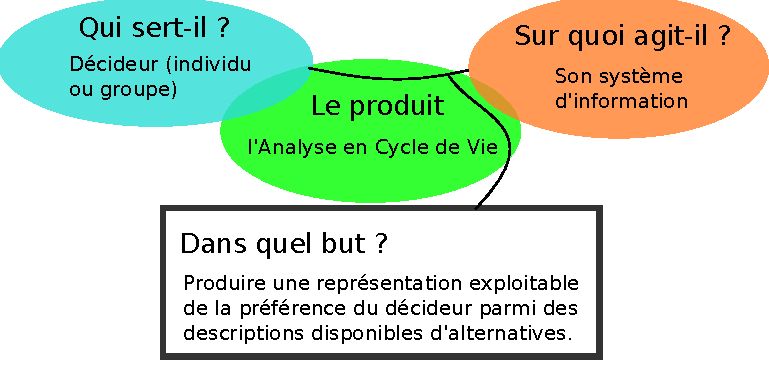
\includegraphics[width=0.7\linewidth]{/home/rudy/Documents/rudy/01_These/11_production/01_COMMUNICATION/figures/bete_a_cornes_201606.pdf}
\caption{Le schéma du besoin pour l'\gls{ACV}.}
\label{fig:diagramme_besoin}
\end{figure}

\figbox{                  
L'application du schéma du besoin à l'\gls{ACV} et la lecture de la figure~\ref{fig:diagramme_besoin}, nous donne l'expression du besoin fonctionnel suivante~:

Notre produit : l'\gls{ACV}, sert le décideur en agissant sur son système d'information dans le but de produire une représentation exploitable de la préférence du décideur parmi des descriptions disponibles d'alternatives.
\footnote{La notion de préférence est traitée au chapitre~\ref{chap:Méthodes et outils} section~\ref{sec:ADMC}, les interacteurs sont décrits dans la discussion suivante.}
}

\subsubsection{Discussion du Besoin}
%Discutons cette lecture pour en sonder ses limites.
L'\gls{ACV} établit une représentation de la préférence qu'aurait un décideur entre des différents états des aires de protection.
Les flux (échanges de produits et substances entre acteurs et milieux) modifient les états (impacts, dommages, satisfactions de fonctions),
\textit{cf.} le descriptif de l'\gls{ACV} \ref{sec:La pensée en cycle de vie}.
\paragraph{Réalisation d'inventaire.}
Questionnons nous à savoir si l'\gls{ACV} comprend ou non la réalisation des descriptions des flux, des systèmes et d'états.
Notons que nous ne pouvons déclarer de préférence vers des alternatives techniques ou organisationnelles que sur la base de leurs descriptions existantes.
C'est à dire que l'information disponible \emph{détermine} la préférence et potentiellement le choix du décideur.
\exbox{
Sur la base de 3 éléments d'information identiques, le classement des alternatives 'a' et 'b' donne $a P b$, (a est préféré à b).
%\marginpar{?notation symbolic logic}
Ces mêmes alternatives a et b sur la base de 4 éléments d'information peuvent parfaitement donner la préférence inverse $b P a$.

Prenons l'illustration de l'achat d'une paire de chaussure 
Vous ordonnez selon votre préférence les paires de chaussures A, B et C.
\begin{itemize}
\item Démarrons avec pour système de dimensions initial~: le système de fermeture, la couleur, la marque. L'ordre est alors~: CAB.
\item Introduisez le prix et l'ordre devient BCA car vous jugez C et A ``trop chères''.
\item Introduisez maintenant la pointure et l'ordre devient ABC où d'ailleurs BC vous sont inutiles car pas à votre pointure.
\end{itemize}
Cette exemple illustre que la valeur des critères (importance relative) conditionne le résultat.
}
\keybox{Il peut donc y avoir la nécessité d'acquisition de données (réalisation d'inventaires) pour répondre au système de valeur du décideur.}
\paragraph{Support de la décision.}
Nous soulignons également la prépondérance donnée au caractère décisionnel de l'\gls{ACV}.
Nous relevons en littérature la dichotomie entre \gls{ACV} de comptabilité et \gls{ACV} de décision.
Cette distinction y est à la fois mentionnée comme~:
\begin{itemize}
\item importante

\blockcquote[p.114, sec.2]{tillman_significance_2000}{Avec une distinction servant la différenciation entre étude rétrospective (comptabilité) et prospective (modélisation des effets du changement).}
%retrospective and prospective, or LCA with an accounting perspective and LCA modeling the effects of changes.
%The distinction between accounting LCAs and change-oriented LCAs is important.
%}
\item et comme artificielle

\blockcquote{weidema_application_1998}{puisque toute production d'information vise à affecter une décision}.
%It may also be argued that the distinction is artificial since the purpose of any information ultimately is to affect a choice, even for such a seemingly "neutral" application as "product declarations".}
\end{itemize} 
%Although it may be argued that all types of LCA are done with the same general purpose (i.e., environmental improvement, which in turn implies change), not all LCAs are made to support decision-making directly, in the sense of choice between formulated alternative actions. Decision-making may be described generally as a procedure where (1) a problem is formulated, (2) alternatives are formulated, and (3) a choice is made between alternative solutions to the problem [1]
%ref non accessible :
% Baumann H. Decision Making and Life Cycle Assessment. Licentiate thesis. Go ̈teborg:
%Chalmers University of Technology. Technical Environmental Planning Report 1995:4.
%(Also available as AFR Report 77. Stockholm: Swedish Waste Research Council.)


%argument court
%\begin{center}\colorbox{yellow}{Trouver formulation pour}\end{center}
%
%-
%
%Lors de ce type d'échange, je pense aux comptables et à leurs 'analyses'...
%"Ah, vous qui travaillez uniquement pour analyser.
%Ce n'est évidement pas pour que ces analyses servent à des décisions ultérieures."
%
%+
%
%L'information est dépendante de son contexte.
%Si je dis, ce produit vaut $35$ euros.
%Vous pouvez prendre cette donnée sur la base d'un consommateur et juger l'information acceptable.
%Si vous êtes parmi les industriels de la chaîne de valeur, ce n'est pas \textit{35} qui vous intéresse, mais $34.85$, car traitant de l'objet à des millions d'exemplaires, les décimales font valeur.
%L'information doit donc être lié à son contexte d'évaluation, son contexte de décision.
%
%-

\citeauthor{tillman_significance_2000} reconnaît d'ailleurs que 
%\footnote{
\blockcquote{tillman_significance_2000}{toutes les applications de l'\gls{ACV} visent le changement}.
%All these applications aim at change, or improvement: some in more direct ways (decision-making), some in more indirect ways, such as influencing market behavior or identifying improvement possibilities.}
%}.
La relations de la méthodologie de l'\gls{ACV} à son application est étudiée de longue date.
Elle réside dans le contexte décisionnel~\cite{wenzel_application_1998}.
%\footnote{
%\blockcquote{wenzel_application_1998}{The need to differentiate the LCA methodology when used in different applications derives from a limited number of variables. These variables all derive from differences in the consequence and the context of the decision to be taken.}
%}.
Puisqu'il y a donc reconnaissance d'une décision, directe ou indirecte, observons le point obtenant une reconnaissance commune~: \emph{l'évaluation}.

L'é\emph{valuation} est l'application d'un jugement de \emph{valeurs} sur des observations.
Or,\blockcquote[traduction]{gasparatos_embeded_2010}{dans la plupart des cas, le choix de l'outil d'évaluation est fait par le ou les analystes sans prendre en considération les valeurs des parties prenantes concernées.}
%In most cases, the choice of the evaluation tool is made by the analyst(s) without taking into consideration the values of the affected stakeholders.
%}
La séparation de l'évaluation et du processus de décision (et donc du décideur~: porteur du jugement) introduit d'après \citeauthor{grahl_evaluation_1996} une \textbf{contradiction}~:
%\footnote{
\blockcquote{grahl_evaluation_1996}{L'évaluation ne peut pas être déléguée en elle même. Si elle était déléguée sans le processus de prise de décision, une évaluation objective (i.e. sans jugement de valeur) serait requise -- une évidente contradiction dans ces termes.}
%The evaluation cannot be delegated on its own. If it were delegated without the decision-making process, an objective (i.e. value-free) evaluation would be required - an evident contradiction in terms.
%}
\label{grahl_impossible_deleguation}
Notez que nous distinguons délégation et séparation.
\exbox{Un couple visite des maisons en vue d'un achat.
La femme du couple, en technicienne avertie
 même si au chômage, 
% vient d'avoir une très bonne impression sur 
%préférera
apprécie une première visite
 d'un bien spacieux, dont les canalisations sont accessibles dans des vides techniques, où l'électricité vient d'être refaite aux normes et
 où seule la décoration reste à faire.
%  dont pour le coup toute la décoration est à faire puisque les murs sont nus dû aux récents travaux.
%Lors de la visite suivante, 
L'homme, %qui brûle de pouvoir enfin s'acheter sa demeure
grâce au poste en CDI dont il vient de valider la période d'essai, se projette 
%complètement 
lors d'une visite dans une charmante petite et \textit{ancienne} maison, avec son sol ancien, son parquet\ldots %et même la petite balancelle avec parasol sous la pergola où il s'imagine berçant l'enfant qu'il souhaite pour devenir Père.
%Il est maintenant hors de question pour lui de repenser 
%L'homme ne peut imaginer
%une contre-visite de ce qui lui est apparu comme un chantier poussiéreux et sans cachet qu'il a vu plus tôt.
%La femme pour ce second bien n'a que faire des sols dont elle sait devoir se défaire car le tout à l'égout n'est pas installé.
%Face à un bien où seul la décoration reste à faire, cette seconde maison \textit{ne vaut rien} (pour elle).

Hors de toute considération d'itérations ou contre-visite et si le décideur est le payeur, ce n'est pas la femme et son système (reste-à-faire, espace, fonctionnalité) mais l'homme qui actera, suivant le système (cachet de l'ancien, décoration, ``ressenti'').

%L'évaluation de madame peut être tout à fait exacte face à son système de valeur (travaux, reste-à-faire, fonctionnalité).
%Toutefois, s'ils avaient à signer dans la seconde et si \emph{le} décideur, avec pour système, le cachet, la décoration, ``le ressenti'' devait apposer son accord, c'est sur le second bien qu'il se lancerait.

Système de valeurs évaluateur et système de valeurs décideur ne font qu'un.}

Nous affirmons, comme \citeauthor{grahl_evaluation_1996},
que l'é\textbf{valua}tion n'est pas \textbf{séparable} des \textbf{valeurs} et donc du \textbf{décideur} (porteur des valeurs qui acte le choix).
Mais nous développerons ultérieurement notre proposition afin de permettre la \emph{délégation} (\ref{délégation de valeurs2}).

Terminons donc par la phrase conclusive de \citeauthor{grahl_evaluation_1996} sur cette question~:
\keybox{
\blockcquote[traduction]{grahl_evaluation_1996}{Les \gls{ACV} sont donc des aides à la prise de décision, mais pas un substitut aux décisions elles-mêmes.
%LCA's are thus a decision-making aid, but no substitute for the decisions themselves
}
}

Il en résulte l'\textbf{expression du besoin}, à remplir par l'ACV~:
\keybox{
Produire une \underline{représentation exploitable} de la \underline{préférence du décideur} (personne ou groupe) parmi des \underline{descriptions disponibles d'alternatives}.
}
Les groupes nominaux (soulignés) de cette phrase seront les éléments clefs de la contribution de ce mémoire.
Les descriptions disponibles traitent de la disponibilité de la données, de sa mise en formes pour un traitement dans le volume nécessaire (Chap.~\ref{chap:Recherche Libre}).
Les représentations exploitables sont celles issues des techniques d'\gls{ADMC}, qui visent à rester dans nos capacités cognitives.
La préférence du décideur est l'objet que nous intégrons dans l'\gls{ACV} par nos travaux, d'abord avec ce qui fut jusqu'ici positionné dans l'étape d'inventaire (i.e. allocation Chap.~\ref{chap:Multifonctionnalité}), puis de façon générale dans l'interprétation (Chap.~\ref{chap:Jugements et Multi-dimensionnalité}).

%{\color{BlueViolet} Our product, or artifact : LCA,} serves {\color{SkyBlue}its user (human for now)} acting on {\color{Goldenrod}the information system} in order to produce a representation of preferences between alternatives according to the decision makers (human) value system.

% \tikz[baseline=(n1.base)]{\node[fill=green!20,rectangle] (n1) {Our product, };}\tikz[baseline=(n1.base)]{\node[fill=green!20,rectangle] (n1) {or artifact : LCA};} serves \tikz[baseline=(n1.base)]{\node[fill=green!20,rectangle] (n1) {its user (human for now)};} acting on \tikz[baseline=(n1.base)]{\node[fill=green!20,rectangle] (n1) {the information system};} in order to produce a representation of preferences between alternatives according to the decision makers (human) value system.

\subsection{Analyse fonctionnelle du besoin (\acrshort{AFB})}
Après avoir clairement identifié le besoin, il faut ensuite décrire en termes de services les nécessités (exigences) pour y répondre.
Il s'agit de \emph{nécessité} au sens large.
\exbox{Ainsi seuls les produits fabriqués (et donc ceux que l'on peut produire), ou naturellement existant, délivrent leurs services.
De même, un produit ne permettant pas le traitement des ses déchets en fin de vie obstruerait et pourrait dégrader nos sociétés.
%Ce qui à termes entraînerait son abandon.
Mais les nécessités réglementaires ou culturelles sont à prendre en compte également.
Imaginez un grill de bœuf en Indes, ou des cendriers de bureau après la loi Évin en France.}
\keybox{
C'est donc la même logique, en cycle de vie et multi-dimensionnelle, qui parcours l'\gls{ACV} et l'\gls{AF}.
}
\subsubsection{Identification des phases de vie du produit}
Usuellement cette étape de l'\gls{AFB} démarre par la distinction des phases de vie du produit.
S'agissant d'une méthodologie nous distinguons les phases suivantes~:
\begin{itemize}
\item Élaboration (conception)
\item Utilisation (application)
\item Fin de vie (fin d'exploitation, obsolescence)
\end{itemize}

Parce que nous sommes dans l'élaboration et que nous n'envisageons pas de dispositif post ACV, nous concentrerons l'étude à l'étape d'utilisation.
Permettons nous toutefois de passer synthétiquement sur ces autres étapes.

L'\textbf{Élaboration} concerne notre travail même.
Cette étape comprend donc dans son milieu extérieur la communauté contribuant à la méthodologie de l'\gls{ACV}.
Nous réfléchissons donc à l'établissement d'une méthodologie de décision visant plus de rationalité et donc un encrage dans notre connaissance du réel dans son périmètre le plus étendu possible (holisme\footnote{Qui considère les objets observés comme un tout.}).
\blockcquote[traduction]{lenoir_curricular_2015}{Plus largement, c'est une indication d'une orientation de nos sociétés occidentales, [\ldots]
%plus que l'émergence de cette orientation:
Ce n'est pas l'émergence d'une façon d'aborder la connaissance de plus en plus divisée, mais plutôt le signe d'une préférence pour la prise de décision éclairée, basée sur des vues techniquement fondées, et sur la volonté de prendre des décisions sur la base des scénarios étayées par des connaissances spécifiques.
Voilà pourquoi l'interdisciplinarité trouve des points d'ancrage dans toutes les sciences appliquées, sociales ou autres. (Sinacœur, 1983, pp. 25-26)}
%More broadly speaking, it is an indication of an orientation of our Western societies, more than the emergence of this orientation:
%It is not the emergence of a way to address increasingly separated knowledge, but rather the sign of a preference for informed decision making, based on technically founded views, and on the desire to make decisions on the basis of scenarios underpinned by specific knowledge. This is why interdisciplinarity finds anchoring points in all the applied sciences, social or other. (Sinacœur, 1983, pp. 25-26)
%}

Il s'agit d'établir les fondations méthodologiques d'une méthode d'évaluation pour la décision (science de gestion) holistique (spectre complet des sciences naturelles), dans la limite des capacités cognitives humaines (neuro-psychologie) et respectueuse du jugement de valeur du décideur (socio-psychologie) applicable à diverses cultures et par elles (sociologie - anthropologie - linguistique).

Il s'agirait donc pour la conception la plus robuste de l'\gls{ACV}, que l'ensemble des disciplines et acteurs mis en œuvre soient sollicités.
%C'est pour partie l'explication de l'étalement disciplinaire de ce mémoire. % traitement des ajouts du 20/06 à zotero
C'est l'un des points de l'argumentaire sur la disponibilité de la donnée (de toutes les disciplines et donc sans barrières entre-elles).

Le milieu extérieur de cette étape comprend également les praticiens actuels.
Nous relevons un conflit d'intérêt important pour les acteurs économiques dont la \emph{reproduction}\footnote{Au sens marxiste du terme, la reproduction des forces de travail.} tient dans la capacité à vendre des prestations d'\gls{ACV} à d'autres acteurs.
Il nous paraît conflictuel à la fois, de produire des réflexions sur une méthodologie comportant plusieurs problèmes non résolus à chacune de ses étapes et de vendre l'application, ou des données pour l'usage, de ladite méthodologie.
Malgré tout, les praticiens les plus expérimentés (et donc à même de juger l'opérationnalité de l'artefact reconçu), sont ceux-là même qui applique la méthodologie actuellement déficiente et qui donc sont psychologiquement et économiquement dans la position la plus délicate pour la remettre en question.

La \textbf{Fin de Vie} de l'\gls{ACV}.
Sur les conditions d’obsolescence de la méthodologie de l'\gls{ACV}, nous ne pouvons que conjecturer sur les évolutions du système d'information, des décideurs, de leur capacités cognitives et de notre organisation sociale face aux choix.
Nous nous abstiendrons de développer ces questions.

Nous observons toutefois que l'étude d'une décision apparaît lorsqu'elle est prise, mais également après, en justification ou plus ultérieurement encore, pour la comprendre.
Cette dernière raison, celle de l'historien nous concerne peut-être peu, si ce n'est que pour demander à ces spécialistes les problèmes qu'ils anticipent dans la compréhension pour les générations futures de nos décisions passées.
C'est à dire ``Que devons nous anticiper relativement à l'élaboration méthodologique de l'\gls{ACV} pour que nos enfants puissent (i) s'en saisir (ii) juger effectivement la méthode obsolète ?''.
Nous ne connaissons pas par avance le contenu qui sera produit.
Cependant, ici encore, il s'agira d'argument en faveur de la \emph{libre} transmission des connaissances pour les générations futures.

Nous poursuivons donc la démarche avec l'étape d'\textbf{Utilisation}.

\subsubsection{Caractérisation en phase d'utilisation de l'\acrshort{ACV}}
\label{subsubsec:Caractérisation ACV}

\paragraph{Identification et caractérisation des \acrlongpl{EME}}

\subparagraph{Distanciation à la représentation classique de l'\gls{ACV}.}
\label{par:Distanciation à la représentation classique de l'ACV}
Nous retrouvons dans les \acrlongpl{EME}, des éléments centraux tels que le décideur et le système d'information mentionnés à l'étape précédente.

Nous avons bien entendu pensé au système de représentation classique de l'\gls{ACV} et du développement durable (\textit{cf.} section~\ref{sec:La pensée en cycle de vie}).
Toutefois la mention d'\gls{EME} comme écosystème, ressources économiques, sphère sociale, ne nous paraissait pas opportune.
En effet, nous considérons que l'\gls{ACV} inter-\emph{agit} avec un système d'information et non ces éléments pré-cités.
L'\gls{ACV} ne touche pas directement les produits, services ou procédés,
car elle n'est pas en contact avec le système observé.
Elle n'est en liaison qu'avec l'information relative au système observé.
Ainsi, l'élément d'interaction est ici le système d'information.

Il est apparu délicat de dissocier la méthodologie de l'\gls{ACV} et le système d'information nécessaire à la réalisation de l'\gls{ACV}.
La question est de savoir si le système d'information est un \gls{EME}.
Or, ce sont bien les caractéristiques méthodologiques de l'\gls{ACV} qui imposent un certain système d'information.
Les caractéristiques précises n'en seront que la traduction en solutions fonctionnelles puis techniques.

Les éléments cités précédemment (\gls{technosphere}, \gls{biosphere}\ldots) ont une forte présence dans la perception actuelle de l'\gls{ACV}.
%Nous tenons donc à permettre au lecteur de visualiser le traitement de cette question.
%Il nous semble donc important de détailler ce point.
%Pour cela nous l'invitons à consulter 
La figure \ref{fig:information_sys},
représentation du système technique, social, économique, vise à proposer une articulation moins simpliste que l'actuel dichotomie technosphère écosphère.
Nous y questionnons notamment la position du système d'information. % ainsi qu'à illustrer le rapport de ces objets au système d'information.

\begin{figure}[htbp]
\centering
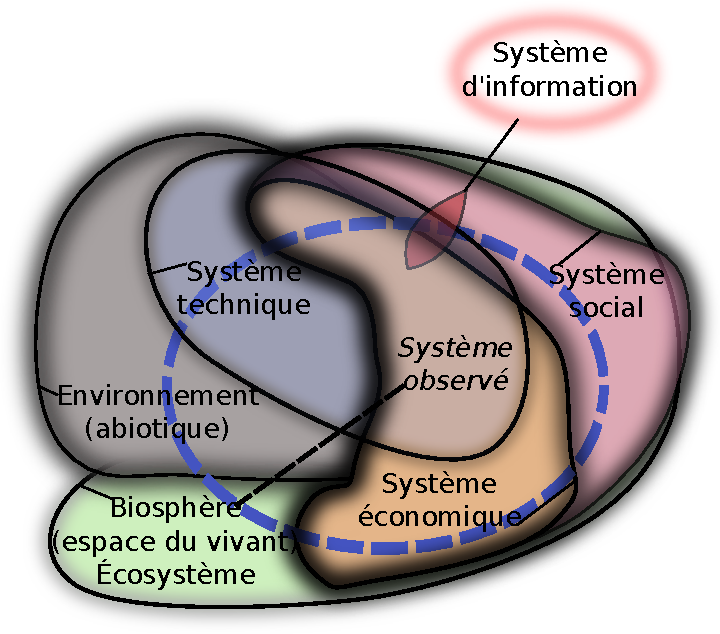
\includegraphics[width=0.7\linewidth]{/home/rudy/Documents/rudy/01_These/11_production/01_COMMUNICATION/figures/systeme_d_information_et_ACV.pdf}
\caption{Représentation alternative pour l'\gls{ACV} des systèmes, techniques, sociaux, économiques et de l'écosphère.}
%Second step in external functional analysis, listing the elements of the artifact's environment and describe its relations trough functions. Either users i.e. functional requirements of constrains. Here only use phase is considered.

\label{fig:information_sys}
\end{figure}

\figbox{
Sur la figure \ref{fig:information_sys}, on observe les différents éléments habituels relatifs à l'\gls{ACV} et décrit à la section~\ref{subsubsec:Vocabulaire de base}~: La biosphère, l'écosphère, la techno-sphère ; mais aussi le vocabulaire des méthodes d'impacts~: les ressources abiotiques, biotiques, l'environnement social.
Un trait relie le périmètre et sa désignation.
Ni les contours, ni les libellés n'ont vocation ici à être exactes.
Ils ne servent qu'à pousser au questionnement.
\exbox{Existe-t-il une part du système technique, qui ne serve pas la répartition des ressources ($\overline{\mathit{système~économique}}$)? , qui ne traite pas des relations entre individus ($\overline{\mathit{système~sociale}}$)?\ldots}
%Nous employons le flou pour indiquer l'incertitude épistémologique et la transparence des surfaces indique la non exclusion des domaines entre eux.

Cette représentation comprend volontairement pour le système observé un contour pointillé et de périmètre inférieur aux différents ensembles, techniques sociaux et environnementaux.
La transparence des surfaces indique la non exclusion des domaines entre eux
En effet, une des difficultés de l'\gls{ACV} est de ne pouvoir traiter que du champ connu des systèmes sans connaître la proportion de cette part dans ces systèmes.
Ces \textit{extérieurs au domaine connu} sont représentés avec un contour flou signifiant notre incertitude épistémologique\footnote{\href{http://www.uved.fr/fileadmin/user_upload/modules_introductifs/module3/risques/1.3/html/2.html}{Hyperlien vers la documentation des formes d'incertitude}.}.

La frontière commune du système social et économique vise à souligner que l'organisation des relations humaines, en général ou en particulier pour la gestions de ressources (économie), repose sur un même et unique encrage matériel.

Au sein de l'\emph{écosphère} l'homme s'est organisé en \emph{société} et a déployé des \emph{systèmes techniques}.
Une partie de ce système socio-technique (vivant et non-vivant, matériel) est le système d'information.
Nous considérons le système d'information comme la combinaison des systèmes techniques (incluant de ressources abiotiques) et de systèmes sociaux (comprenant les personnes -- compris dans l'écosystème -- travaillant au sein de celui-ci), visant l'information.

%L'homme observant l'écosphère ainsi que lui même produit l'observation.
Le système observé est la fraction de l'écosphère inscrite au système d'information.
%Toutefois toutes les données relatives au système d'information ne sont pas nécessairement incluses à l'information dans ce système.
Le système d'information n'observe donc qu'une partie de l'écosphère, du système socio-technique et de lui même.
\emph{C'est cette partie qui est exploitable pour la prise de décision.
Il ne faut donc pas oublier de quels composants (humains et techniques) elle découle.}

Une fois rendu plus souples dans nos perceptions catégorisées de notre environnement, nous pouvons franchir l'étape suivante.
La décision affecte par partie ou dans son ensemble les différents systèmes entremêlés.
Qu'importe qu'il s'agisse d'un espace que l'on qualifie d'éco-bio-techno-sphère, que les éléments affectés soit biotique ou non.
Des états sont modifiés, les étiquetages qu'il est possible de réaliser ne doivent servir qu'à l’assistance du décideur pour 'situer' sa préférence.
%C'est sur elle que porte l'évaluation.
% texte des différents domaines
%Ressources non employées dans les systèmes techniques
%Y a-t-il des systèmes techniques ne servant pas à la gestion de ressources ?
%Vide si l'on considère les ressources pour le système technique.
%Système de gestion des ressources (non uniquement monétaire)
%L'écosystème (biotique et abiotique) observé fait-il nécessairement part du système sociale ou non ? Nous partons sur le principe que non.
%Commerce du vivant (agriculture, sylviculture, élevage, travailleurs)
%Un système technique peut-il être hors de notre système sociale ? Une épave de navire
%Vide suivant que l'on considère le domaine du vivant avec ou sans son support matériel
%Vide pour ceux de croyance athée.
%? noosphère
%\begin{center}
%\colorbox{yellow}{Trouver un formalisme sur la symbolique des ensembles ?}
%\end{center}
%
%$homme \in vivant \in biosphère \in ecosphère$
%
%$ecosphère - biosphère = abiotique$
%
%$système technique = $
%\end{tcolorbox}
}
Cette représentation complexe est simplifiée pour la figure~\ref{fig:octopus_LCA}.
Il n'y a, par exemple, dans cette seconde figure pas d'intersection entre système technique et écosystème (biosphère).
Or tout système agricole comprend des outils (abiotique) et des outils vivants (biotique)\footnote{Le terme dans ce cadre est `auxiliaire de culture'}.
Cette représentation doit toutefois déjà nous éclairer pour dépasser notre dichotomie classique \Gls{technosphere} | \Gls{ecosphere}.

\subparagraph{Les \gls{EME} de l'\gls{ACV}} considérés sont donc pour cette étape "utilisation" et sur cette base de l'interaction avec un système d'information, les \gls{EME} de la figure~\ref{fig:EME-ACV}.
\begin{figure}[h]
\centering
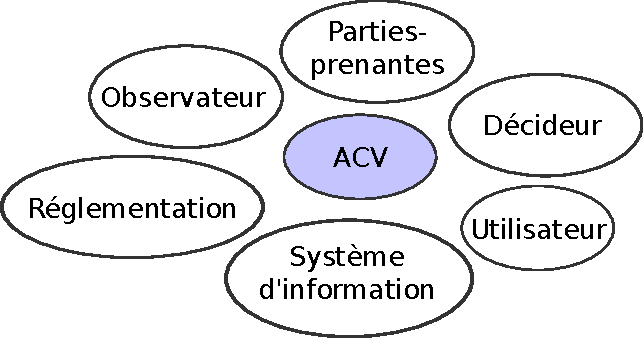
\includegraphics[width=0.8\linewidth]{/home/rudy/Documents/rudy/01_These/11_production/01_COMMUNICATION/figures/EME.pdf}
\caption{Éléments du Milieu Extérieur de l'\gls{ACV} en phase d'utilisation.}
\label{fig:EME-ACV}
\end{figure}
\figbox{
Le schéma des EME de notre application est la représentation fig.~\ref{fig:EME-ACV}.
Ce type de schéma comprend généralement~: l'utilisateur, l'observateur, la réglementation, la matière d'œuvre et le milieu environnant.
Nous omettons volontairement ce dernier (environnement). celui-ci conduit aux fonctions de résistance au milieu (usuellement caractéristiques de corrosion, résistance UV\ldots).
Ce choix réside dans le fait que nous n'éclairons pas les caractéristiques géographiques et matériels en support à la méthodologie (réseaux de communication, appareillages).
Nous ne faisons pas ici l'\gls{AF} du matériel d'un système d'information supportant l'\gls{ACV} mais celui de la méthodologie de l'\gls{ACV} elle-même.
Ceci implique que notre caractérisation portera sur la méthode et les caractéristiques du traitement de l'information (logique, cognition, mathématiques, légales\ldots) et pas sur la condition matérielle de l'application de l'\gls{ACV} (data-center, nature des réseaux de communication, volume de données, vitesses de calculateurs\ldots).
%Nous comprenons cependant l’existence de limites techniques quant à la capacité de calcul et de stockage requise.
%Mais ces éléments sont simplement hors de notre champ de compétences.

Ainsi pour notre analyse, les EME sont~: La réglementation, l'observateur, les parties-prenantes, le décideur, l'utilisateur et le système d'information.
%Nous serons amener à faire évoluer ces représentations au fil du travail.
}
\paragraph{Identification des Fonctions de Services (F.S.)}
Analysons maintenant les relations entre l'\gls{ACV} et ses EME.
Cette analyse est facilitée par la représentation graphique du diagramme des interacteurs, figure~\ref{fig:octopus_LCA}.
%dans ces phases de vie.
Ceci nous guide dans l'identification des fonctions que doit remplir l'\gls{ACV} et la définition de ses caractéristiques consécutives.
%Then analyzing the relation between LCA (our artifact) and its environment, trough the octopus graph~\ref{fig:octopus_LCA}, guides us toward the characteristics such tool shall possess.


\begin{figure}[htbp]
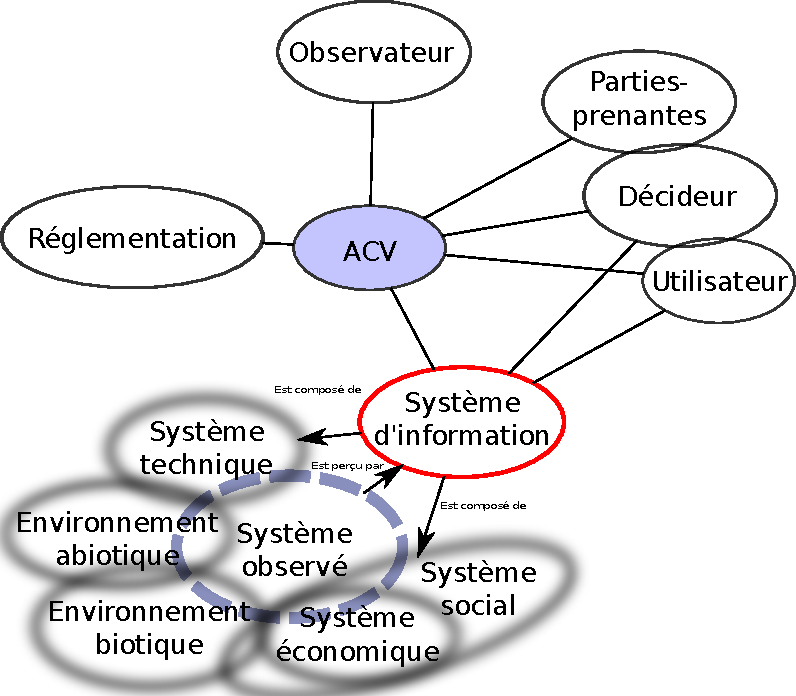
\includegraphics[width=\linewidth]{/home/rudy/Documents/rudy/01_These/11_production/01_COMMUNICATION/figures/octopus_ACV.pdf}
\caption{Représentation des éléments de l'environnement du produit en interaction avec lui (phase d'utilisation).
%Second step in external functional analysis, listing the elements of the artifact's environment and describe its relations trough functions. Either users i.e. functional requirements of constrains. Here only use phase is considered.
}
\label{fig:octopus_LCA}
\end{figure}

\figbox{
La figure~\ref{fig:octopus_LCA} est lu de la façon suivante.
Nous débutons par une représentation des éléments classiques de l'environnement incluant la réglementation, l'observateur et l'utilisateur.
Chacun exerce à minima une contrainte sur l'objet à concevoir, représentée par un trait simple fig.~\ref{fig:octopus_LCA}.

Deux \gls{EME} agissent sur la matière d’œuvre, l'utilisateur et le décideur.
Nous commençons par lier d'un trait droit ces \gls{EME} et le système d'information.
La suite de la caractérisation déterminera la nature de ces relations lorsque nous préciserons en quoi l'ACV modifie ces liaison entre acteurs et matière d'œuvre\footnote{Puisque nous sortons du cadre classique des représentations d'\gls{AF}, nous pouvons souligner qu'il pourrait être intéressant d'illustrer d'autres relations entre \gls{EME}, par exemple l'interaction entre des parties-prenantes et la réglementation.
Lors de recherche ultérieures, cela apportera peut-être de nouvelle thématiques de recherche, comme des pratiques de conception.}.
}

Nous allons donc observer et \textbf{décrire chaque \gls{EME}} puis détailler les relations à l'\gls{ACV}.
Ces observations nous permettrons ensuite de \textbf{formuler des exigences fonctionnelles} pour la caractérisation des fonctions de l'\gls{ACV}.
Les exigences seront listées indépendamment de leur redondance à d'autres \gls{EME}.
\exbox{Être compréhensible, d'un observateur comme de l'utilisateur par exemple.}
Une exigence fortement redondante est normalement adressée avec une plus forte priorité.
Ceci se traduit par des niveaux plus strictes des critères relatifs à ces fonctions.
%If we detail the relationship between LCA and its environment we can state the following elements.

\subparagraph{Le Système d'information}
\label{subparagraph:Le Système d'information}
\subparagraph{Description de l'inter-acteur~:}

Nous avons développé la représentation relative au système d'information figure~\ref{fig:information_sys}, car c'est un élément central.
\emph{Parce que le système observé est vaste, dynamique, global et complexe, le système d'information est (devrait être) à son image.}
Nous tendons à diviser le système observé en techno-sphère, biosphère en système social et économique.
Ce faisant, nous oublions qu'il ne s'agit que d'une seule et même réalité.
Cette représentation est donc une construction arrangeante pour la comptabilisation de flux au travers de frontières.
Le volume de contrôle déterminé par l'interaction humaine visait à identifier des flux élémentaires (générateur d'impact) et des flux produits établissant la chaîne de valeur.
Or, des indications sont observées à la fois dans et hors du volume de contrôle.
De plus, la caractérisation des impacts nécessite une localisation plus fine que "rejet dans la biosphère".
Ceci est observé à travers la sous-compartimentation déjà existante et croissante, disponible en méthodes d'impacts et dans les travaux sur la spatialisation~\cite{yan_ontology_2015}~:
eau~: douce, marine ; air~: forte densité de population, faible densité de population \ldots
%\begin{itemize}[noitemsep,topsep=0pt,parsep=0pt,partopsep=0pt]
%\item eau
%\begin{itemize}[noitemsep,topsep=0pt,parsep=0pt,partopsep=0pt]
%\item douce
%\item marine
%\end{itemize}
%\item air
%\begin{itemize}[noitemsep,topsep=0pt,parsep=0pt,partopsep=0pt]
%\item forte densité de population
%\item faible densité de population
%\end{itemize}
%\item sol
%\end{itemize}
%\ldots

Nous ne devrions pas rester prisonniers d'une partition d'un système que nous avons nous même établi.
Il faut alors comprendre et accepter la multitude de perceptions du système dans lequel nous somme immergé.
Cela peut être le résultat d'une multitude d'opinions issues d'une même perspective culturelle ou par l'intégration d'une multitude de perspectives culturelles.
Il faut donc laisser à l'utilisateur de la méthode d'\gls{ACV} et aux développeurs la possibilité de déterminer les caractéristiques du(des) volume(s) de contrôle.
Si un décideur considère plus importante une région géographique particulière, les caractéristiques méthodologiques de l'\gls{ACV} (dans ses normes comme ses outils) ne doivent pas y faire obstacle car ce serait faire obstacle au système de \emph{valeurs} à appliquer et donc à l'é\emph{valuation}.


\subparagraph{Exigences~:}
 
 Les attributs de la structure de connaissances, du système d'information utilisé doivent être~:
 
 \begin{itemize}[noitemsep,topsep=0pt,parsep=0pt,partopsep=0pt]
  \item Adaptabilité. Doit pouvoir être adapté aux écarts linguistiques et culturels, donc permettre le traitement de multiples ontologies.
  \item Interactivité. Doit être caractérisé par l'absence ou la limitation la plus importante possible de barrières et couloirs d'étranglement à la production, la mise à jour et la correction.
  \item Robustesse. Doit être équipé des outils les plus avancés de manipulation et sauvegarde des données et de leurs versions.
  \item Globalité. Doit être développé avec de multiples standards de communication. Doit être accessible et fourni à travers le globe et éditable depuis chaque endroit.
  \item 'Scalablilité'. Doit permettre de faire face au gigantisme de la masse d'information à traiter. %la lisibilité par machine en vue
  \item De complétude minimale. Doit contenir l'ensemble de l'information minimum à l'exercice de la fonction de l'\gls{ACV}.
  Ici nous devons disposer \emph{à la fois} les descriptions objectives et des valeurs (opinions) avec une distinction claire des deux natures d'information stockées.
 \end{itemize}


%\begin{description}
% \item Information system:
% 
% LCA does not touch the products, services, processes.
% LCA is not in contact with the system observed.
% Its relates to information about the observed system.
% So the element LCA interacts with, is the information system.
% We developed it here because it is a central element.
% And as the observed system is vast, dynamic, global, complex, the information system is (must be) to its image.
% We tend to divide the observed system in techno-sphere, biosphere, social, economical systems.
% And doing so we start to forget it is a single one reality.
% It is a convenient construction in order to account flows to rise borders.
% But we should not remain entangled within one perceived partition of the system.
% We must also comprehend the varying perception of the system.
% May it be with wide-ranging opinions from the same cultural perspective or by the integration of wide-ranging cultures.
 
% Requirement:
% 
% The knowledge structure and information system used must be:
% \begin{enumerate}[noitemsep,topsep=0pt,parsep=0pt,partopsep=0pt]
%  \item Versatile. That can be adapted to mind the language or cultural gaps and encompass multiples ontologies.
%  \item Highly interactive. Limited or absence of up-dating and correcting bottle neck(s).
%  \item Robust. Equipped with state-of-the-art versioning management and safeguards tools.
%  \item Globalized. Developed with multiples and/or widely used communication standard, globally accessible and locally supplied all around the globe.
%  \item Scalable, machine readable (to face the gigantism of data to handle).
%  \item Withhold both descriptions and value systems with clear distinction.
% \end{enumerate}

%   \end{description}


\subparagraph{La Réglementation~:}
 \subparagraph{Description de l'inter-acteur~:}
 L'\gls{ACV} manipule des données.
 En conséquence, cet outil doit conduire au respect des droits d'auteurs et diverses propriétés relatives à ces informations.
 L'\gls{ACV} a une forte intensité en données qui nécessitent de pouvoir être utilisées, modifiées, distribuées, pour la vérification et curarisation.
 Ces opérations doivent pouvoir se faire avec le moins de résistance possible, résistances légales incluses, sans pour autant contrevenir aux législations.
 
% Ces notions sont éclairées par le travail de \citeauthor{beitone_biens_2010}.
% Il nous faut les appliquer aux éléments manipulés en \gls{ACV}.
% L'\gls{ACV} agit sur les systèmes d'information, pas autre chose.
% Les conditions appliquées à ces informations, leur « licence », déterminent ce qui peut être fait de l'\gls{ACV}.
% 
% \begin{tabular}{ p{5cm} p{5cm} p{5cm}}
% 	\hline
% 	& Excluabilité & Non excluabilité \\
% 	Rivalité & Biens privatifs & Biens communs \\
% 	Non rivalité & Biens de club & Biens collectifs \\
% 	\hline
% \end{tabular}
% 
% Comme les lecteurs l'auront constaté en état de l'art, les biens de club sont la majorité en \gls{ACV}.
  
 Le traitement des informations qui portent sur les préférences et opinions, nécessite la protection des personnes qui les expriment.
 \emph{Il est également nécessaire d'apporter une protection contre l'unification et la standardisation des systèmes de valeurs comme outil d'hégémonie, par exemple~: l'obligation légale d'application d'un système de valeurs unique identifié.}\footnote{Sans quoi nous ne respectons pas l'ensemble des composants de la définition de soutenabilité, \textit{cf.} Sec.~\ref{sec:La Soutenabilité}.} %(http://www.cnrtl.fr/lexicographie/h%C3%A9g%C3%A9monie)
  
 %
 % \item Regulations:
 % 
 % LCA handles data.
 % So a legitimate consequence is that using LCA must respect authors properties rights.
 % LCA being data intensive, it needs to be able to use, modify and distribute a lot of data with as less resistance as possible.
 % The diffusion of information on preferred values (and as a results systems) generate protections or weaknesses.
 % Protection against unification or standardization of value systems as hegemonic weapons should be carefully studied.
 % What would be the consuming behavior with alternative regulation on supplementary information ?
 % As an example, try to picture your reaction with \ref{fig:declaration_soutenable_pdt}.
 
\exbox{
 Nous illustrons l'étude de cet \gls{EME} avec les déclarations environnementales de type III\footnote{Les déclarations environnementales actuelles sont déclinées en I écolabels, ISO~14024 (certification)~;
 II auto-déclaration, ISO~14021 (déclaration à la responsabilité du producteur)~;
 III éco-profils ISO~14025, communication de résultats d'ACV.}.
 Faisons l'hypothèse d'une réglementation rendant obligatoire le type d'affichage proposé dans le modèle ATLETTE II (Appliance Testing for Washing Machines Energy Label \& Ecodesign Evaluation)~\cite{therese_kreitz_atlete_2014}.
 Quel serait le comportement de consommateur avec une réglementation alternative sur l'information complémentaire obligatoire sur les produits de grande consommation (propositions fig.~\ref{fig:declaration_soutenable_pdt})~?
 }
 
 Une personne prend naturellement (sans assistance) un mode de raisonnement heuristique~\cite{meyer_modetraitement_2000}.
 C'est à dire qu'une sélection de l'information employée pour la décision est opérée sur la base de l'expérience (des pré-jugés) de la personne.
 Ceci dans le but de réduire l'énergie consommée, le coût cognitif.
 \blockcquote{meyer_modetraitement_2000}{Nous traitons l'information la plupart du temps selon un principe de moindre effort (Allport, 1954) et de suffisance
 (Simon, 1976) par rapport aux buts du traitement.}
 
 Les habitudes des consommateurs traitent nécessairement du prix et ses variations.
 Un affichage traitant des notions habituelles, non-techniques et émotionnellement liées aux sujets, pourrait avoir une influence bien plus importante sur son choix.
 Nous ne limitons d'ailleurs pas nos hypothèses d'application au EuP-ErP (produit utilisateur d'énergie ou lié à l'utilisation d'énergie).
 Nous reprenons donc dans un premier exemple pour illustrer ce propos, les travaux de Gaël \textsc{Gireau} (facteur 12)~\footnote{Ces travaux traitent de l'encadrement des salaires. Ce type de questionnement en économie à d'ailleurs fait l'objet d'une votation en Suisse~\cite{chancellerie_federale_suisse_votation_2013,gadrey_ecarts_2013}}.
 Un étiquetage visant la soutenabilité pourrait par exemple reprendre l'écart salarial sur l'ensemble de la chaîne de valeurs (supply chain).
 Ainsi, imposer non pas une contrainte salariale mais commerciale (publier l'écart des salaires), pourrait (ou non) conduire à un resserrement des rémunérations.
 
 Dans un second exemple, nous pourrions employer un indicateur "social" avec des niveaux de risques indiqués sur le travail des enfants~\cite{benoit-norris_identifying_2012,wang_analytic_2016, dreyer_characterisation_2010} (ex : de la Social Hotspot Database SHDB).
 L'implication émotionnelle de l'acheteur--\emph{euse} envers la mise au travail des enfants aurait certainement une influence plus forte qu'un indicateur technique aux ordres de grandeur non employés par le consommateur
 \footnote{D'autant plus pour la population féminine encore majoritairement en charge des courses et des enfants~\cite{ricroch_en_2012}.
 }.
 
 \begin{figure*}[htbp]
   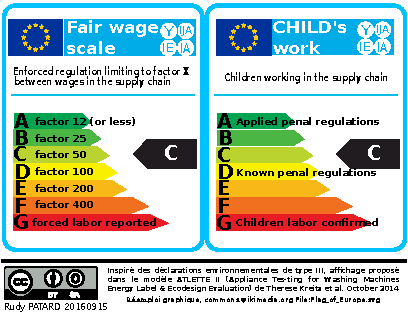
\includegraphics[width=\textwidth]{/home/rudy/Documents/rudy/01_These/11_production/01_COMMUNICATION/figures/declaration_soutenable_pdt_A.pdf}
   \caption{Visions alternatives de l’étiquetage environnemental et durable.
   Quelle information supplémentaire donner aux consommateurs pour guider leur choix~?
   Proposition basée sur ATLETE II~\cite{therese_kreitz_atlete_2014}}
   \label{fig:declaration_soutenable_pdt}
 \end{figure*}
   
 \figbox{
Dans la figure~\ref{fig:declaration_soutenable_pdt}, nous proposons des alternatives d'affichage hypothétiques sur la base du modèle ATLETTE II.
Partant de lidée d'illustration de la proposition initial des auteurs \citeauthor{therese_kreitz_atlete_2014}, sur une échelle de classe de consommation d'énergie, nous proposons des graphiques alternatifs.
L'illustration à gauche est une proposition basée sur l'écart salarial au sein de la chaîne de valeur.
L'illustration de droite propose l'affichage d'une échelle sur le travail des enfants dans la chaîne de fournisseurs.
}
\keybox{Nous le voyons donc, la reconnaissance de l'intérêt public dans l'accès à une information ou sa reconnaissance comme faisant partie du domaine privé conditionne la capacité à réaliser de l'ACV.
Ceci implique que tant qu'une information jugée privée\footnote{Dans les exemples il s'agit de la distribution des salaires et de l'âge dans la chaîne de valeur.} est nécessaire à l'ACV, un équivalent ouvert, mentionnant les écarts possibles et hypothèses attenantes doit être produit.}

  
\subparagraph{Exigences~:}
 \begin{itemize}[noitemsep,topsep=0pt,parsep=0pt,partopsep=0pt]
  \item Les orientations des licences sur les données et outils doivent libérer ces derniers des contraintes du droit d'auteur et de la propriété intellectuelle, justement pour ne pas les enfreindre.
  Pour toute donnée fermée l'équivalent ou substitut ouvert doit être produit avec la plus grande ouverture et transparence.
  Les licences employées doivent laisser un maximum de liberté à la création, modification, distribution des données, codes et résultats. 
  
  \item Le système doit lever toute limitation en terme de système de valeur. Ainsi, il doit gérer l'inconsistance \emph{au sein des} systèmes de valeurs et \emph{entre les} systèmes de valeurs, sans être une imposition de valeurs contraire à la réglementation.
  
  \item Le système doit protéger les déclarants sur l’énoncé de leurs jugements.\footnote{
  Lié à la question de la liberté d'opinion, de ton et de parole, au plan international, il s'agit d'un point sensible.
  Il doit être défini de façon claire sur les modalités de transparence et d'espace privé.
  Pour une personne morale, où considérons nous qu'une information privée portant sur des dangers pour d'autres, devrait ou non être révélée au public~?
  }.
 \end{itemize}
 
%
% Requirement:
% \begin{enumerate}[noitemsep,topsep=0pt,parsep=0pt,partopsep=0pt]
%  \item So the chosen regulation under which put the data and tools must be clearly selected toward this goal: free-open.
%  \item Allow no value system limitation.
%  So handle inconsistencies within value systems.
%  \item Protection on personal judgments declaration\footnote{It is linked to the theme of freedom of opinion and freedom of speech. Here must also be chosen the side between transparency and privacy. Where do we consider that private information but harmful to all should not be disclosed?}.
% \end{enumerate}
% 
\subparagraph{L'Observateur--trice~:}
\subparagraph{Description de l'inter-acteur~:}
 Avant même d'être utilisateur de l'\gls{ACV} ou de ses résultats, une personne peut être observatrice de l'outil.
 Il a été souligné au \ref{sec:La pensée en cycle de vie} que la question de la légitimité et de la confiance en l'\gls{ACV} est un point essentiel pour qu'elle soit considérée et employée (i.e. que des personnes deviennent utilisateur et décideur comme nous le verrons ensuite).
 Plus l'outil apparaîtra comme obscure, inconsistant, moins il apparaîtra comme sûr et digne d'intérêt.
 Pour qu'un observateur considère l'information fournie par l'\gls{ACV} comme valide, crédible et légitime, la méthode et son application doivent être transparentes. Ceci est nécessaire pour assurer la confiance de l'observateur dans la capacité d'une prise de décision au delà de nos limites cognitives actuelles, cf. sec~\ref{sec:ADMC}.
% L'\gls{ACV} doit gagner en légitimité et en crédibilité par plus de transparence et assurant la confiance dans la capacité d'une prise de décision au delà de nos limites actuelles~\ref{label}.

 En plus des outils et données ouvertes (spécifiés dans les exigences sur le système de données), apparaît ici la nécessité d'information complémentaire de vulgarisation.
 L'\gls{ACV} n'est pas limitée à ceux qui la pratiquent.
 Elle doit pouvoir, lorsqu'elle est observée, être comprise par ceux qui potentiellement et à des degrés divers la subissent. %garde-t-on subir ?
 
%\colorbox{yellow}{Trouver un // sur l'information du consommateur sur les subst.dangereuses.}
%
%\colorbox{yellow}{Confrontation du thème de la publicité et de l'information.}
%
%
%
%\colorbox{yellow}{obstacle à l'intervensionisme de l'utilisateur dans le système de valeur}
 \subparagraph{Exigences~:}
 \begin{itemize}
 \item Une vulgarisation progressive doit être disponible pour tout observateur.
 \item La \textbf{distinction} entre \textbf{faits} et \textbf{opinions} doit être \textbf{systématique} pour assurer la confiance au futur décideur potentiel dans l'application de \emph{son} système de valeur\footnote{Nous retrouvons des conséquences classiques en conception relative à `l'observateur', qui se résume à~: attirer l'utilisateur potentiel.}.
 \end{itemize}
 
 
 \subparagraph{L'Utilisateur--trice~:}
 \subparagraph{Description de l'inter-acteur~:}
 Ici, nous considérons l'utilisateur de l'\gls{ACV}.
 Il s'agit donc de l'entité qui modélise et qui calcule l'\gls{ACV}.
 Ceci peut être perçu comme le praticien (LCA practitionner).
 L'utilisateur de l'\gls{ACV} n'est pas nécessairement, le décideur.
 
 Il s'agit ici de prendre à contre-pied \emph{`l'impossible délégation'} de l'évaluation de \citeauthor{grahl_evaluation_1996} section \ref{grahl_impossible_deleguation}.\label{délégation de valeurs2}
 L'utilisateur doit produire un résultat dans un cadre décisionnel (comme vu section \ref{subsec:besoin}).
 S'il n'est pas possible de produire une évaluation sans le système de valeurs du décideur, il n'est pas interdit de faire appliquer ledit système par un tiers.
 \textit{De facto}, il s'agit donc d'une délégation de l'évaluation mais pas un changement de décideur.
 En effet, nous pouvons rendre possible la délégation de l'évaluation par la \emph{transmission du système de valeur du décideur à l'utilisateur}.
% Soit pour une décision directe, soit pour la fourniture d'une information exploitable lors d'une décision ultérieure\footnote{Distinction des cas de décision suivant l'ILCD, Table "Study types"\cite{european_commission_ilcd_2010}}.
 Le cadre méthodologique de l'\gls{ACV} doit donc permettre au praticien de s'extraire des jugements appliqués, sans ambiguïté.
 L'utilisateur devant répondre au décideur suivant son contexte de décision, la temporalité de l'évaluation ne doit pas dépasser celle de l'action de décision.
 Dans un temps limité, l'utilisateur doit donc produire une représentation compréhensible d'une préférence entre alternatives sur la base d'une grande étendue d'informations (bis repetita des arguments du point relatif au système d'information~\ref{subparagraph:Le Système d'information}). % centaines, miliers d'info (3000 substance, 8000 procédés, plusieurs dizaines d'indicateurs et leurs agrégations)
  \subparagraph{Exigences~:}
 \begin{itemize}[noitemsep,topsep=0pt,parsep=0pt,partopsep=0pt]
  \item L'\gls{ACV} doit présenter de façon lisible et compréhensible son processus et ses résultats.
  \item L'\gls{ACV} doit prendre en compte les limites cognitives humaines durant son processus et employer des méthodes et outils permettant de dépasser nos limites de rationalité.
%  \marginpar{? \textbf{Cosmin}, quelle contradiction}
  \item L'\gls{ACV} doit apporter une réponse pour la prise de décision dans le cadre temporel de la décision, \emph{sans y mêler le jugement de l'utilisateur} lorsque celui-ci diffère du décideur.
 \end{itemize}
% \item Observer:
% 
% Before using LCA or its resulting information, a person can observe LCA.
% It has been pointed out that LCA must earn its legitimacy to be considered a proper tool for decisions. (RETROUVER LA SOURCE)
% The more obscure or inconsistent, the less secure and interesting the tool appear.
% LCA must gain in legibility and transparency to secure trust and confidence in the decision it enables.
% 
% Requirement:
% 
% On top of open access to data and tools (specified with information system requirements), the information must be presented with force of vulgarization, consistence.
% The distinction between facts and opinion shall be systematic.
% 
% \item User:
% Here we specify a user of LCA.
% This entity is the one that models and calculates.
% It can be seen as the LCA practitioner.
% It is not (necessarily\footnote{
% Apart for those doing LCA for their own decision.
% A reality that could arise sooner than we anticipate.})
% the user of the result of LCA.
% 
% Requirement:
% \begin{enumerate}[noitemsep,topsep=0pt,parsep=0pt,partopsep=0pt]
%  \item The LCA must present human readable conclusion and process.
%  \item It must respect human cognitive limits or apply methods and other artifact to exceed them.
% \end{enumerate}


\subparagraph{Le Décideur~:}
\label{decideur}
 \subparagraph{Description de l'inter-acteur~:}
 \blockcquote[traduction]{murray_transdisciplinary_2015}{Les normes d'ACV identifient directement différents décideurs institutionnels, y compris l'industrie (développement de produits, le marketing, la planification stratégique) et le gouvernement (politique publique), mais les consommateurs et les citoyens ne sont pas directement mentionnés. En revanche, le consommateur est un centre d’attention d'une économie axée sur la demande et les préférences des consommateurs, des orientations et des visions du monde valeur informent des discussions LCA de valeurs (par exemple Hofstetter et al., 2000).}
% LCA standards directly identify various institutional decision makers including industry (product development, marketing, strategic planning) and government (public policy), but consumers and citizens are not directly mentioned. In contrast, the consumer is a focus of a demand-driven economy and the consumer’s preferences, value orientations and worldviews inform some LCA discussions of values (e.g. Hofstetter et al. 2000).
% }
 
   Le décideur (individu ou groupe) soumet son/ses systèmes de valeurs pour que la solution qui sera sélectionnée corresponde à ce système de valeurs.
   Qu'il(s) choisisse(nt) d'être en nombre limité (mona-oliga-rchie), ou de distribuer plus largement la déclaration de préférences,
   le décideur \emph{doit avoir la maîtrise du système de valeurs employé} dans cette expression de l'é\emph{valuation}.
   L'apport primordial du décideur à l'\gls{ACV} est le système de valeur.
   Il doit pouvoir se consacrer à son expression et faire que celle-ci soit la plus exploitable.
   En considérant que les valeurs d'un individu stable le sont également, le système de valeurs doit être applicable indépendamment du contexte (donc de l'application).
      
 \subparagraph{Exigences~:}
 
 L'\gls{ACV} doit permettre
 
 \begin{itemize}[noitemsep,topsep=0pt,parsep=0pt,partopsep=0pt]
  \item l'intégration du système de valeurs du décideur (individu ou groupe)~;
  \item le contrôle par le décideur de l'application de son système~;
  \item l'obtention d'une représentation de sa préférence envers les alternatives qui lui soit accessible (disponible et compréhensible)~;
  \item la protection du décideur dans sa déclaration d'opinions, \emph{si celle-ci doit pouvoir rester privée}~;
 \end{itemize}
% \item Stakeholders:
% 
% This category is large.
% We specified a user and an observer category for their specificities.
% Who are those concerned with the applications of LCA (``Product development and improvement, Strategic planning, Public policy making, Marketing, Other''\cite[Figure 1 Framework for life cycle assessment (from ISO 14040:2006; modified)]{european_commission_ilcd_2010})?
% I could discern two subcategories\footnote{These subcategories are not disjoint. But the range of consequences is not necessarily uniformly distributed among the discussed categories.}:
% \begin{itemize}[noitemsep,topsep=0pt,parsep=0pt,partopsep=0pt]
%  \item Decision maker(s) (causal party)
%  \item Decision affected parties (consequence party)
% \end{itemize}
% If we are to apply a tool with such an important impact in terms of application, we shall consider the political implication in terms of governance.
% The decision maker(s) submitting her/his/their value system for their preferred solution to be selected chose to either be in limited number (oligarchism) or to distribute the declaration of preferences.
% In a case where those suffering the negatively perceived consequences are not those beneficing the positively perceived ones debating who rightfully claim the preference system to be applied is of prime importance.
% This also imply that the communication of information must be done so that it reflect the decision maker(s) selection.
% For democratic context, a complete vulgarization and systematic progressive explanation is necessary.
% 
% Requirement: LCA must provide
% \begin{enumerate}[noitemsep,topsep=0pt,parsep=0pt,partopsep=0pt]
%  \item Consistence between political perspective(s) and implementation of value systems of stakeholders.
%  \item Wide sets of representations accessible (that can be reached and understood) to all stakeholders.
% \end{enumerate}
 
\subparagraph{Autres parties prenantes~:}
 \subparagraph{Description de l'inter-acteur~:}
 
%  C'est ici une large catégorie.
  Les utilisateurs, décideurs et observateurs sont spécifiés pour leurs particularités.
  Il convient maintenant également de traiter ceux qui seront concernés par l'application de l'\gls{ACV} (``Product development and improvement, Strategic planning, Public policy making, Marketing, Other''\cite[Figure 1 Framework for life cycle assessment (from ISO 14040:2006; modified)]{european_commission_ilcd_2010}), sans qu'ils fassent usage de l'\gls{ACV}, soient à l'origine du système de valeurs employé ou sans même  qu'ils observent l'un (le système de valeur) ou l'autre (l'\gls{ACV}).
  Deux sous-catégories de parties-prenantes sont discernées~:
  \begin{itemize}[noitemsep,topsep=0pt,parsep=0pt,partopsep=0pt]
   \item Décideur(s), (Decision maker(s)) (partie causale), traitée précédemment,
   \item Parties affectées (partie conséquence)
  \end{itemize}
  Ces sous-catégories ne sont pas disjointes.
  Mais la plage de conséquences n'est pas nécessairement uniformément distribuée sur ces catégories.
  Il peut être avancé qu'un décideur, ayant intégré une plus grande part d'information, notamment relative aux conséquences, puisse agir sur des décisions personnelles conduisant à une moindre exposition aux conséquences négatives et/ou à une plus grande exposition aux bénéfices des choix actés
  \footnote{Question du délit d'initié.}.
  Si nous appliquons un tel outil avec des conséquences importantes en termes d'applications (\textit{cf.} la section relative aux applications de l'\gls{ACV}~\ref{sec:La pensée en cycle de vie}), nous devons prendre en compte les \emph{implications politiques en terme de gouvernance}.
   
  Dans un cas où ceux subissant les conséquences perçues négativement ne sont pas ceux bénéficiant des conséquences perçues positivement, débattre de qui peut légitimement déterminer quel système de valeurs sera appliqué est de première importance.
  Ceci implique également, en termes de communication, que le message (s'il en est un de diffusé) doit inclure la façon dont a été déterminé le \emph{système de valeurs décisionnaire} (la sélection du décideur).
  \exbox{
  Pour reprendre notre exemple de l'affichage environnemental (figure \ref{fig:declaration_soutenable_pdt}), celui-ci devrait donc porter une explication du système de valeur employée. Exemple, une mention du type : panel européen à intervalle de confiance de 95\%
%  \marginpar{\textbf{voir Cosmin}}
%  \marginpar{"Il porte déjà (parfois)"}
  adjoint à une localisation pour l'accès et l'observation de ce système de valeur (ex~: une URL).
  }
  Une partie prenante par voie de conséquence doit pouvoir devenir observatrice sous les gouvernements qui en juge ainsi de l'information des citoyens.
  
  Dès-lors qu'une partie prenante peut introduire son propre système de valeur en substitution de celui employé pour l'évaluation, elle devient le décideur.
  \exbox{
  ex: hypothèse du développement d'une application, soit mobile par QR-code, soit sur ordinateur pour le e-commerce, qui reproduit l'affichage suivant le système de valeur du consommateur).}
  Les exigence de ce groupe s'appliquent alors cf. (\ref{decideur}) inter-acteur précédent.
  \subparagraph{Exigences~:}
  
  L'\gls{ACV} doit fournir~:
  
  \begin{itemize}[noitemsep,topsep=0pt,parsep=0pt,partopsep=0pt]
   \item une \textbf{consistance} entre le cadre politique et l'implémentation des systèmes de valeurs des parties prenantes\footnote{Ex~: Une décision publique dans un cadre démocratique emploie le système de valeurs du peuple auquel s'applique la décision.}~;
   \item une large gamme de représentations du système de valeurs appliqué, accessible à l'\emph{ensemble} des parties prenantes, accessible dans ses deux acceptions, qui peut être \emph{atteinte} et \emph{comprise}.
  \end{itemize}
  


\paragraph{Caractérisation des Fonctions de Service (F.S.)}

%\paragraph{Synthèse des exigences fonctionnelles}
Reprenant les interacteurs, nous identifions un certain nombre de fonctions récurrentes, issues des exigences.
À la suite de plusieurs itérations de reformulation des exigences, nous obtenons une liste réduite de fonctions de services. %, principale et contraintes (en réponse au besoin extérieur et imposées par l'environnement pour obtenir le service).
%\marginpar{\textbf{Cosmin}{\tiny J'ai repris les brouillons pour écrire les tables de reformulation. Mais même en annexe je ne trouve pas qu'elles aient leur place}.}
L'objectif de la première phase de cette étape est d'obtenir la liste minimale des fonctions à caractériser.
Cette liste est reprise table~\ref{tab:ACV-fonctions}.


%\begin{longtable}{p{2.5cm}|p{2cm}|p{8cm}}
%inter-acteur & libellée & fonction \\
%\hline
%
%Le système d'information & FC1 & L'ACV doit être adapté aux écarts linguistiques et culturels.\\
%Le système d'information & FC2 & L'ACV doit permettre le traitement de multiples ontologies.\\
%Le système d'information & FC3 & L'ACV ne doit pas comporter de barrières ou couloirs d'étranglement à la mise à jour et à la correction.\\
%Le système d'information & FC4 & L'ACV doit s'inscrire dans les versions des observations.\\
%Le système d'information & FC5 (FC1' FC2') & L'ACV doit être développée avec de multiples standard de communication.\\
%Le système d'information & FC6 & L'ACV doit être accessible et fourni à travers le globe et éditable depuis chaque localité.\\
%Le système d'information & FC7 & L'ACV et son contenu doivent être lisibles par machine.\\
%Le système d'information & FC8 & L'ACV doit contenir à la fois les descriptions objectives et les valeurs et opinions.\\
%Le système d'information & FC9 & L'ACV doit permettre une distinction claire des deux natures d'information stockées~: objectif et subjectif.\\
%
%Réglementation & FC10 (FC3') & L'ACV doit reposer sur des licences permettant librement la modification, l'utilisation, transmission.\\
%Réglementation & FC11 (FC1') & L'ACV doit lever toute limitation en terme de système de valeur.\\
%Réglementation & FC12 (FC2') & L'ACV doit gérer l'inconsistance au sein des systèmes de valeurs et entre les systèmes de valeurs.\\
%Réglementation & FC13  & L'ACV doit employer un système d'information qui protège les déclarants sur l’énoncé de leurs jugement.\\
%  
%Observateur& FC14 (FC1') & L'ACV doit comporter une vulgarisation progressive et disponible à tout observateur (FC1-FC2).\\
%Observateur& FC15 & L'ACV doit assurer sa propre crédibilité.\\
%Observateur& FC16 (FC9') & L'ACV doit permettre la distinction systématique entre faits et opinions. RQ : moyen à FC15.\\
%
%Utilisateur& FP1 & L'ACV doit présenter de façon (lisible et compréhensible : FC17), la préférence du décideur envers une série d'alternatives, suivant la globalité de son système de valeurs.\\
%Utilisateur& FC17  & L'ACV doit respecter les limites cognitives humaines durant son processus et employer des méthodes et outils permettant de dépasser ces limites de rationalité.\\
%Utilisateur& FP2 (FP1') & L'ACV doit respecter le cadre temporel de la prise de décision de l'utilisateur.\\
%
%Parties prenantes & FC18 &  L'ACV doit fournir une consistance entre le cadre politique et l'implémentation des systèmes de valeurs des parties prenantes.\\
%Parties prenantes & FC19 (FC6')(FC6' FC14' FC1') &  L'ACV doit fournir une large gamme de représentations accessible (dans ses deux acceptions, qui peu être atteinte et comprise) et cela à l'ensemble des parties prenantes.\\
%\end{longtable}
%
%
%\begin{longtable}{p{2.5cm}|p{2cm}|p{8cm}}
%inter-acteur & libellée & fonction \\
%\hline
%
%Le système d'information & FC1 & L'ACV doit être adapté aux écarts linguistiques et culturels.\\
%Le système d'information & FC2 (FC1') & L'ACV doit permettre le traitement de multiples ontologies.\\
%Le système d'information & FC3 & L'ACV ne doit pas comporter de barrières ou couloirs d'étranglement à la mise à jour et à la correction.\\
%Le système d'information & FC4 & L'ACV doit s'inscrire dans les versions des observations.\\
%Le système d'information & FC6 & L'ACV doit être accessible et fourni à travers le globe et éditable depuis chaque localité.\\
%Le système d'information & FC7 (Moyen FC17') & L'ACV et son contenu doivent être lisibles par machine.\\
%Le système d'information & FC8 (Moyen FP1)& L'ACV doit contenir à la fois les descriptions objectives et les valeurs et opinions.\\
%Le système d'information & FC9 & L'ACV doit permettre une distinction claire des deux natures d'information stockées~: objectif et subjectif.\\
%
%Réglementation & FC10 & L'ACV doit suivre un développement qui limite les contraintes réglementaires s'imposant à elle.\\
%Réglementation & FC13 & L'ACV doit protéger les déclarants sur l’énoncé de leurs jugements, avant et après cet énoncé.\\
%  
%Observateur& FC14 (FC1') & L'ACV doit comporter une vulgarisation progressive et disponible à tout observateur (FC1-FC2).\\
%Observateur& FC15 & L'ACV doit assurer sa propre crédibilité.\\
%Observateur& FC16 (FC9') & L'ACV doit permettre la distinction systématique entre faits et opinions. RQ : moyen à FC15.\\
%
%Utilisateur& FP1 & L'ACV doit présenter de façon (lisible et compréhensible : FC17), la préférence du décideur envers une série d'alternatives, suivant la globalité de son système de valeurs.\\
%Utilisateur& FC17  & L'ACV doit respecter les limites cognitives humaines durant son processus et employer des méthodes et outils permettant de dépasser ces limites de rationalité.\\
%Utilisateur& FP2 (FP1') & L'ACV doit respecter le cadre temporel de la prise de décision de l'utilisateur.\\
%
%Parties prenantes & FC18 (FP1') &  L'ACV doit fournir une consistance entre le cadre politique et l'implémentation des systèmes de valeurs des parties prenantes.\\
%Parties prenantes & FC19 (FC6' FC14' FC1') &  L'ACV doit fournir une large gamme de représentations accessible (dans ses deux acceptions, qui peu être atteinte et comprise) et cela à l'ensemble des parties prenantes.\\
%\end{longtable}

%itération 3 -> reformulation et agrégation
%>> reformulation encours avec les graphes
%


%\begin{longtable}{p{2.5cm}|p{2cm}|p{8cm}}
%libellé initiaux & renumérotation & fonction \\
%\hline
%FP1 & FP1 & L'ACV doit présenter la préférence du décideur envers une série d'alternatives, suivant la globalité de son système de valeurs.\\
%FC17 & FC1 & L'ACV doit respecter les limites cognitives humaines durant son processus et permettre de les dépasser.\\
%%FC8 & FC2 & L'ACV doit contenir à la fois les descriptions objectives et les valeurs et opinions.\\
%FC1 & FC2 & L'ACV doit être adaptée aux distributions géographiques, linguistiques et culturels des parties prenantes.\\
%FC3 & FC3 & L'ACV doit assurer son développement en données.\\
%FC15 & FC4 & L'ACV doit assurer sa validité et crédibilité.\\
%FC10 & FC5 & L'ACV doit suivre un développement qui limite les contraintes réglementaires s'imposant à elle.\\
%FC13 & FC6 & L'ACV doit protéger les déclarants sur l’énoncé de leurs jugements, avant et après cet énoncé.\\
%\end{longtable}

\begin{table}[h]
\begin{tabular}{p{2cm}|p{10cm}}
Libellé & fonction \\
\hline
FS1 & \textbf{Présenter la préférence du décideur} envers une série d'alternatives, suivant la globalité de son système de valeurs.\\
FS2 & \textbf{Respecter les limites cognitives} humaines.\\
FS3 & \textbf{Être adaptée aux distributions culturels}.\\
FS4 & \textbf{Assurer son développement en données}.\\
FS5 & \textbf{Être valide et crédible}.\\
FS6 & \textbf{Respecter les contraintes réglementaires}.\\
FS7 & \textbf{Protéger les déclarants} sur l’énoncé de leurs jugements.\\
\end{tabular}
\caption{Fonctions de l'\gls{ACV}}
\label{tab:ACV-fonctions}
\end{table}



%\colorbox{yellow}{MAJ de la figure avec les nouvelles descriptions de fonction}
%
%\colorbox{yellow}{écart entre \ref{fig:octopus_LCA} et \ref{fig:interacteurs et fonctions}.}


%\begin{figure}[htbp]
%  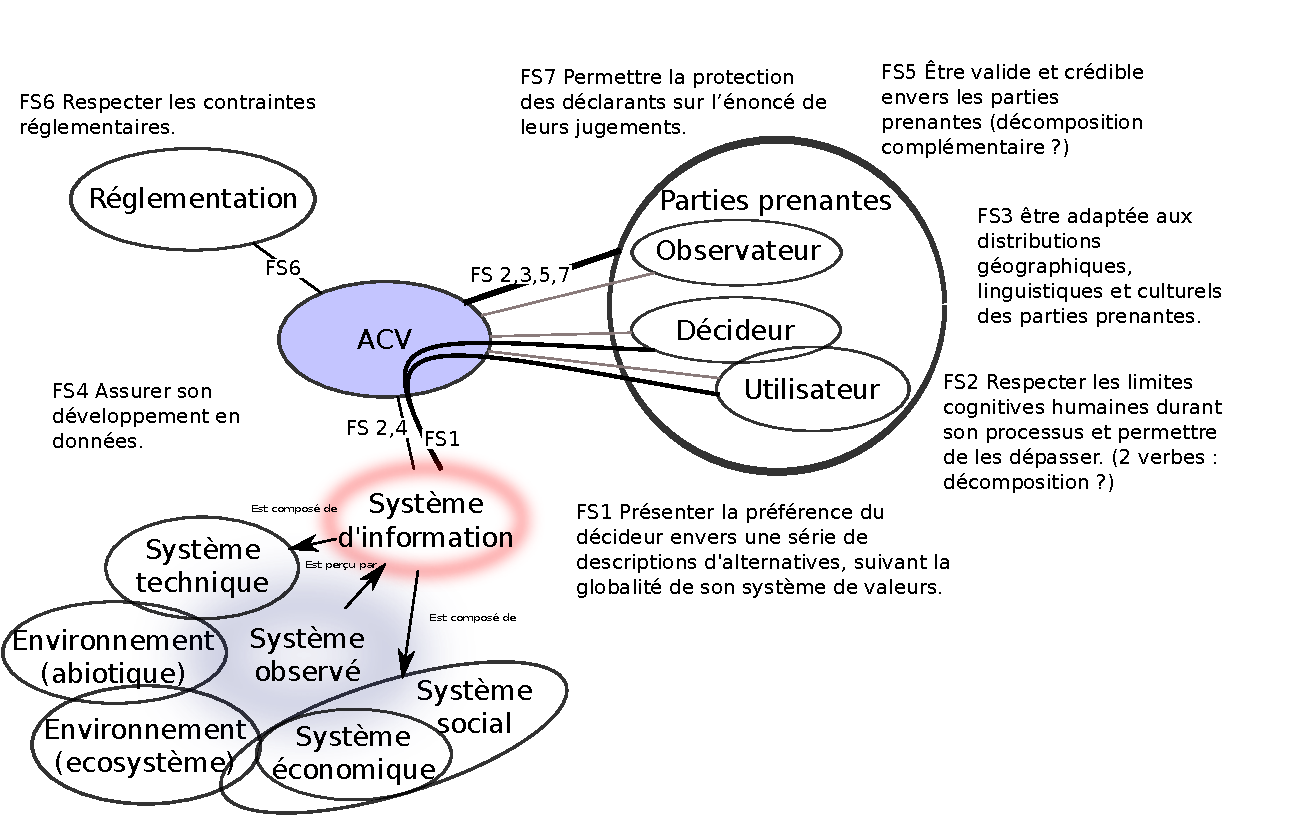
\includegraphics[width=1\textwidth]{/home/rudy/Documents/rudy/01_These/11_production/01_COMMUNICATION/figures/octopus_ACV-ref-fonction.pdf}
%  \caption{Représentation des fonctions sur la graphe des interacteurs. }
%  \label{fig:interacteurs et fonctions}
%\end{figure}
\begin{figure}[htbp]
  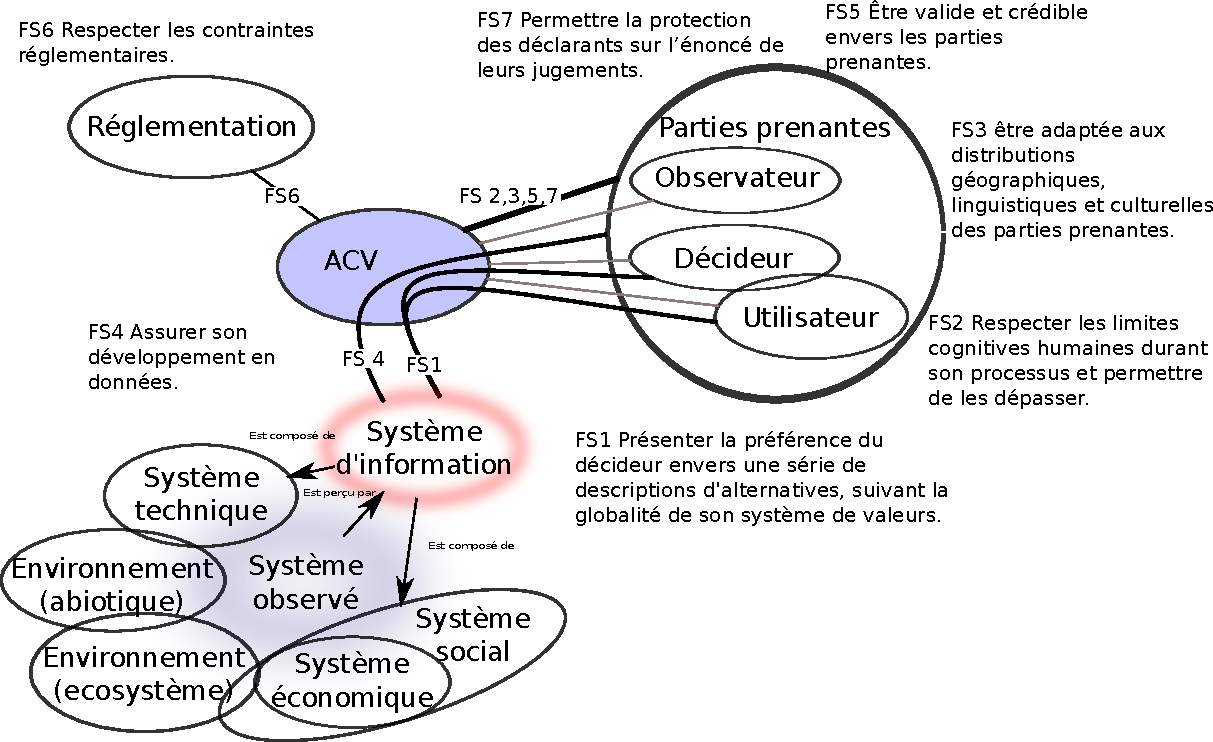
\includegraphics[width=1\textwidth]{/home/rudy/Documents/rudy/01_These/11_production/01_COMMUNICATION/figures/octopus_ACV-ref-fonction_V2.pdf}
  \caption{Représentation des fonctions sur la graphe des interacteurs. }
  \label{fig:interacteurs et fonctions}
\end{figure}
\figbox{
La représentation finale des interactions est donnée figure~\ref{fig:interacteurs et fonctions}.                  
En représentation de diagramme des intéracteurs, les fonctions contraintes sont des traits simples liant \textbf{un} EME au produit.
Les fonctions 'principales' sont représentées par des traits courbes, liant à minima \textbf{deux} EME au produit.

Nous observons qu'une série de contraintes identiques (2,3,5,7) s'appliquent à l'ensemble des parties prenantes, qu'elles soient conservées intégralement ou non dans le groupe 'décideur'.

L'évaluation ne peut pas être faite sans l'interaction du décideur.
Elle peut toutefois être réalisé par l'utilisateur après transmission du système de valeurs du décideur.
Ceci est représenté par le trait courbe en fourche (Système d'information, décideur, utilisateur) signifiant la première fonction de service (FS~1).
}

\subparagraph{Discussion} sur la distinction entre fonctions contraintes et fonctions principales.

La fonction FS~4 met en interaction des parties prenantes et le système d'information au travers l'\gls{ACV}.
Les données d'observations peuvent être d'origine variées (non nécessairement des données d'inventaires spécifiques pour l'\gls{ACV}).
Les données sont produites par des tiers et donc des 'parties prenantes' productrices de données employées en \gls{ACV} contribuent au système d'information (FS~4).
Toutefois des données peuvent ne pas correspondre à ce qui est exploitable dans les méthodes d'impacts. % (\textit{cf.} \ref{} couverture et spécificité de la données).
Il doit donc y avoir des 'ponts de langage' entre les données des parties prenantes hors \gls{ACV} et les méthodes d'impacts (données sur les mécanismes environnementaux).
Définir FS~4 en contrainte ou principale réside dans la distinction entre~:
\begin{itemize}
\item L'\gls{ACV} doit \textbf{exploiter} les croisements d'ontologies \emph{existants} (contrainte du système d'information vers l'\gls{ACV}).
\item L'\gls{ACV} doit \textbf{développer} les croisements d'ontologies des \emph{existantes} (principale~: construction avec les parties prenantes d'éléments de langages communs).
\end{itemize}
Notre perception de l'\gls{ACV} par sa pratique nous pousse à retenir la seconde déclaration.
%\paragraph{Caractérisation des Fonctions de Service}

La distinction entre fonction contrainte et principale nous parait dans d'autre cas moins applicable et exploitable.
Certains cas complexes rendraient les représentations peu exploitables par un grand nombre de ligne courbe perdant le lecteur.
Par exemple, les fonctions FS~2,3,5,7 portent toutes sur l'ensemble des parties prenantes.
Mais elles peuvent très bien être lu comme des liaisons entre plusieurs EME.
Si la FS~7 vise la protection des déclarants (i.e. décideur), elle les protège des autres parties prenantes et reste pour l'observateur une source de confiance dans un futur potentiel emploi de l'\gls{ACV}.
FS~7 se mêle alors à la validité et la crédibilité de la démarche (FS~5-7).
Cette protection peut également s'appuyer de la législation qui s'y rapporte (FS~7-6).
Des clauses particulières peuvent encadrer la relation entre l'utilisateur et le décideurs

La production de confiance (validité, crédibilité, FS5) peut porter (i) du décideur pour lui-même (ii) du décideur vers l'observateur lors d'une décision publique (iii) ou encore de l'utilisateur vers le décideur et/ou l'observateur pour s'assurer de sa non-interférence.

Plutôt que d'alourdir inutilement la figure~\ref{fig:interacteurs et fonctions}, ou de la déclinée dans de multiples versions, nous passons de l'identification à la caractérisation.

\subparagraph{Tables de caractérisation.}
Les tables de caractérisation définissent les modalités selon lesquelles le produit répondra aux fonctions.
Les champs traditionnellement employés sont le libellé de la fonction, les critères observés (entité quantifiée ou qualifiée), le niveau (quantification ou qualification cible), la flexibilité\footnote{Afnor FD X 50-159, fiche O5 "caractériser les fonctions"}.
Nous n'irons pas jusqu'à nous permettre de définir la flexibilité avec laquelle nous souhaitons voir l'\gls{ACV} révisée.
De même nous ne hiérarchisons pas les fonctions entre-elles.
Le but de cette exercice n'est pas tant de donner un cahier des charges pour l'\gls{ACV} mais d'identifier les fonctions de services manquantes à l'état actuel de la méthodologie pour corriger celle-ci.
Nous suggérerons toutefois un certain nombre de critères et de niveaux dans la table~\ref{tab:carac-ACV-fonctions}, sur la base de l'argumentaire développé ci-dessous pour chaque fonction.
%? Niveau Flexibilité  > discussion uniquement des Critères ? proposition de niveau ?

\subparagraph{FS1~:~Présenter la préférence du décideur.}
Il nous semble évident que, si la finalité de l'objet à concevoir et d'appliquer un jugement de valeur à des observations, le jugement de valeur comme les descriptions doivent être respectés.
c.a.d que~:
\begin{itemize}
\item la globalité du jugement doit être employé (pas d'heuristique, 100~\% du jugement émit).
\item toute description utile doit être exploitée (pas de coupure \textit{a~priori}, 100~\% de l'information disponible).
\end{itemize} 
L'implication d'un délai à la restitution de l'évaluation vise encore une fois à marquer l'intégration à un processus de décision.
Suivant chaque contexte décisionnel, il peut s'agir de l'ordre de l'heure (panier d'achat web), de jours (réponse à des fournisseurs) voir de mois ou des années (études de décisions stratégiques, ex: nations, multi-nationales).

\subparagraph{FS2~:~Respecter les limites cognitives}
Les limites cognitives, en termes de nombre d'objets à conserver en mémoire de travail, sont basses (moins de 7 pièces d'information nouvelles et potentiellement jusqu'à seulement 3)~\cite{farrington_seven_2011}.
Il convient donc de limiter ce nombre d'éléments à mémoriser afin de rendre la procédure la plus accessible possible.
Par ailleurs, il n'est pas possible de limiter les dimensions observées (indicateurs), sans faire obstacle à la diversité culturelle potentielle (FS3).
Il ne doit donc pas y avoir de limite théorique que ce soit sur les dimensions observées ou sur les alternatives considérées.

De plus, dans son expression complète nous spécifions pour cette fonction "Respecter les limites cognitives humaine et permettre de dépasser nos limites de rationalité".
En effet pour valider les critères et niveau de FS1 (emploi de la globalité du jugement et des descriptions du système observé), tout en restant sous le seuil de surcharge cognitive, il convient d'attester de la rationalité du jugement mis en œuvre (de sa consistance) et de valider celle-ci comme recevable.
Soit nous posons un seuil de consistance, soit nous considérons l'extraction de la part consistante du jugement~\cite{barzilai_consistency_1998}.
%\footnote{
Ce qui est perturbant dans l'\emph{extraction d'un jugement consistant} d'un jugement inconsistant, c'est qu'il ne peut s'agir \emph{que} d'une déformation du jugement exprimé.
Et sans savoir si cette extraction tend vers le jugement effectif du décideur ou si elle tend vers une meilleur accommodation d'une erreur d'expression du jugement, cela nous parait compliqué de réaliser cette extraction pour un individu unique.
Cette démarche nous semble toutefois parfaitement cohérente avec une logique de décideur multiple (groupe).
Dans ce cas en effet, le jugement du groupe étant une construction, donner l'aval à la partie commune et consistante du jugement d'un groupe semble parfaitement approprié.
%}
\subparagraph{FS3~:~Être adaptée aux distributions culturelles}

Plutôt que d'indiquer langage écrits, nous avons préféré langage 'transcriptible'.
Écrit serait un caractère plus excluant.
Toutefois toute culture non-écrite n'est pas nécessairement transcriptible.
Pour des questions de traçabilité, de capacité de vérification, nous nous limitons cependant aux éléments pouvant laisser une trace écrite.
 %, pouvant être transcrit.
 
Par ailleurs, les décideurs souhaitant intégrer les jugements des parties affectées sur les localisations d'impacts doivent pouvoir intégrer les jugements qui émanent desdites localités.
Il faut noter que ce type de processus nécessitera des déclarations particulières de la part de ces décideurs particuliers pour résoudre les inconsistances potentielles entre le système de valeurs adjoint et le leur.
Il faudrait en effet pouvoir résoudre spatialement l'inconsistance.
Si ce type de cas n'a sans doute pas d'importance pour la décision de personnes physiques, ceci semble capital pour des personnes morales d'envergure internationale (des états et leurs diverses unions, les multi-nationales).

\subparagraph{FS4~:~Assurer son développement en données.}
Comme cela aura été constaté à la sous-section correspondante~\ref{subsubsec:Bases de données}, bien que la qualité et l'accessibilité des données soit le thème récurent des problématique d'\gls{ACV} (cf~\ref{subsec:Problèmes méthodologiques}), le modèle organisationnel choisi jusqu'ici n'offre pas le service requis (nous manquons toujours largement de données).
Pour répondre à la fois à la problématique de responsabilité de l'auteur et d'une plus grande liberté dans l'élaboration et l'utilisation des données, nous considérons l'emploi de licence du \emph{type} CC-BY-SA (créative commons - attribution créditant l'auteur - partage dans les mêmes conditions), comme vu dans l'illustration~\ref{fig:AAA-FR}.

Une fois libéré des contraintes légales et réglementaires par ce choix organisationnel, c'est une caractérisation sur l'échelle du volume à traiter qu'il faut prévoir.
En complément de la mention présente pour FS~1 (exploitation de la totalité des descriptions disponibles), c'est une disposition rendant réalisable cette exploitation qui est nécessaire (la lisibilité par machine).

\subparagraph{FS5~:~Être valide et crédible.}
La validité et la crédibilité d'un outil d'aide à la décision sont des caractéristiques cruciales pour qu'il soit employé.
Sauf à reproduire à l'identique les mécanismes de confiances actuels, classiques, de la publication scientifique en recherche, il ne nous reste plus qu'à ouvrir les comités de revue et les mécanismes de révision eux-même.
Puisque la confiance \textit{hors de la capacité de vérification} tient à celui à qui on l'accorde, les données ne peuvent être inscrites anonymement.
Ceci sera développé au chapitre~\ref{chap:Recherche Libre}.
\subparagraph{FS6~:~Respecter les contraintes réglementaires.}
Nous posons comme évidence le fait de respecter la législation. Pour que l'ACV puisse être applicable, c'est la démarche \textit{active} de placer l'objet hors du champ des contraintes réglementaires qu'il convient d'acter.

Une partie du travail législatif actuel réside dans des accords pour faire sortir d'un domaine propriétaire des travaux des puissances publiques\footnote{À titre d'exemple citons le travail de \textsc{Couperin} sur la \href{https://www.republique-numerique.fr/consultations/projet-de-loi-numerique/consultation/consultation/opinions/section-2-travaux-de-recherche-et-de-statistique/exception-de-fouille-de-texte-et-de-donnees}{fouille de texte}.}.
Afin d'éviter tout obstacle qui rendrait la donnée caduque, obstacles de propriété lucrative notamment (et les diverses formes de propriété intellectuelle qui en sont les instruments), c'est le domaine \emph{libre de droit} qu'il convient de choisir nativement pour les données issue du travail public\footnote{Des travaux tels que ceux sur le génome humain, nous indiquent la voie depuis plus de vingt ans~\cite{pietu_projet_2013}}.
\subparagraph{FS7~:~Protéger les déclarants.}
Comme cela a été souligné à plusieurs reprise déjà, l'\gls{ACV} requière la déclaration d'un jugement de valeur.
L'espace de description objectif étant très vaste, il semble inadéquat de l'envisager hors ligne sauf pour des entreprises disposant de moyens considérables.
Le jugement va donc probablement être appliqué à de la donnée en ligne.
Il convient donc de protéger le déclarant.
Nous envisageons donc que les requêtes au système d'information de l'\gls{ACV} soient réalisées via un réseau d'anonymisation (ex: The Onion Router, TOR \cite{dingledine_tor:_2004,reed_anonymous_1998}).

%\colorbox{yellow}{introduction et conclusion après le tableau qui sont importante}
\subparagraph{Synthèse.}
Comme il est d'usage, nous synthétisons ces éléments dans une table de caractérisation.
Le tableau~\ref{tab:carac-ACV-fonctions}
\begin{table}
\begin{tabular}{p{5cm}|p{4.5cm}|p{4.5cm}}
\textbf{Fonction} & \textbf{Critère} & \textbf{Niveau}\\
\hline
%&&\\
\multirow{4}{*}{\parbox{5cm}{FS1 Présenter la préférence du décideur}} %envers une série d'alternatives, suivant la globalité de son système de valeurs.}}
	& Conformité au jugement du décideur & Identique au jugement émis\\ %\hline
	\cline{2-3}
	& Étendu des descriptions employer & 100\% \\ %\hline
	\cline{2-3}
	& Délai & (suivant cadre décisionnel)\\
%	&&\\
	\hline
\multirow{4}{*}{\parbox{5cm}{FS2 Respecter les limites cognitives humaines}}
	& Nombre d'éléments en mémoire & 3~\cite{farrington_seven_2011} \\ %\hline
		\cline{2-3}
	& Nombre de dimensions considérées & sans limite \\ %\hline
		\cline{2-3}
	& Nombre d'alternatives considérées	 & sans limite \\ %\hline
		\cline{2-3}
	& Seuil d'inconsistance	 & $CR < 0.1$ pour les individus~\cite{saaty_decision_2004}, inconsistance nulle pour les groupes\cite{barzilai_consistency_1998,ishizaka_how_2006}.\\ %\hline
\hline
\multirow{1}{*}{\parbox{5cm}{FS3 Être adaptée aux distributions culturels}}
	& Types de langage considérés & "transcriptible" \\
	&&\\
	\hline
\multirow{5}{*}{\parbox{5cm}{FS4 Assurer son développement en données}}
	& Étendue de la couverture	& Globale\\
		\cline{2-3}
	& Contrainte à la lecture	& Aucune hors infrastructure matérielle\\
		\cline{2-3}
	& Contrainte à l'écriture	& Aucune hors infrastructure matérielle\\
		\cline{2-3}
	& Contrainte à l'utilisation	& Aucune hors infrastructure matérielle\\
		\cline{2-3}
	& Lisibilité machine	& Pour toute donnée quantifiée ou qualifiée\\
	\hline
\multirow{3}{*}{\parbox{5cm}{FS5 Être valide et crédible}}
	& Nombre de revues critiques par donnée	& $\geq3$ ; selon système de valeurs du décideur*\\
			\cline{2-3}
	& Couverture de la revue	& Pluri-nationale ; *IDEM\\
			\cline{2-3}
	& Données Anonymes	& Non\\
	\hline
\multirow{1}{*}{\parbox{5cm}{FS6 Respecter les contraintes réglementaires}}
    & /	& /\\
	&	& \\
%	&	& \\
	\hline
\multirow{3}{*}{\parbox{5cm}{FS7 Protéger les déclarants}} % sur l'énoncé de leurs jugements.}}
	& Utilisation individuelle	& Via réseau de type TOR\\
				\cline{2-3}
	& Dépôt par un tiers pour les outils en lignes	& Systématique\\
				\cline{2-3}
	& Contrôle de la CNIL sur les dépôts	& Systématique\\
	\hline
\end{tabular}
\caption{Ébauche de caractérisation des fonctions de l'\gls{ACV}}
\label{tab:carac-ACV-fonctions}
\end{table}

\subsubsection{Analyse Fonctionnelle Technique}

L'exploration de l'espace des solutions répondant aux fonctions de service peut se faire au travers des diagrammes FAST (Function Analysis System Technique).

Ces diagrammes ont été produits fonction par fonction, tel que présenté en annexe \ref{subsec:FAST}.
Coupant avec les représentations classiques, fonction par fonction, sont représentés ici l'ensemble des éléments de la table~\ref{tab:ACV-fonctions} pour faire ressortir des réponses techniques \emph{communes} aux fonctions de services.

\begin{figure}[htbp]
  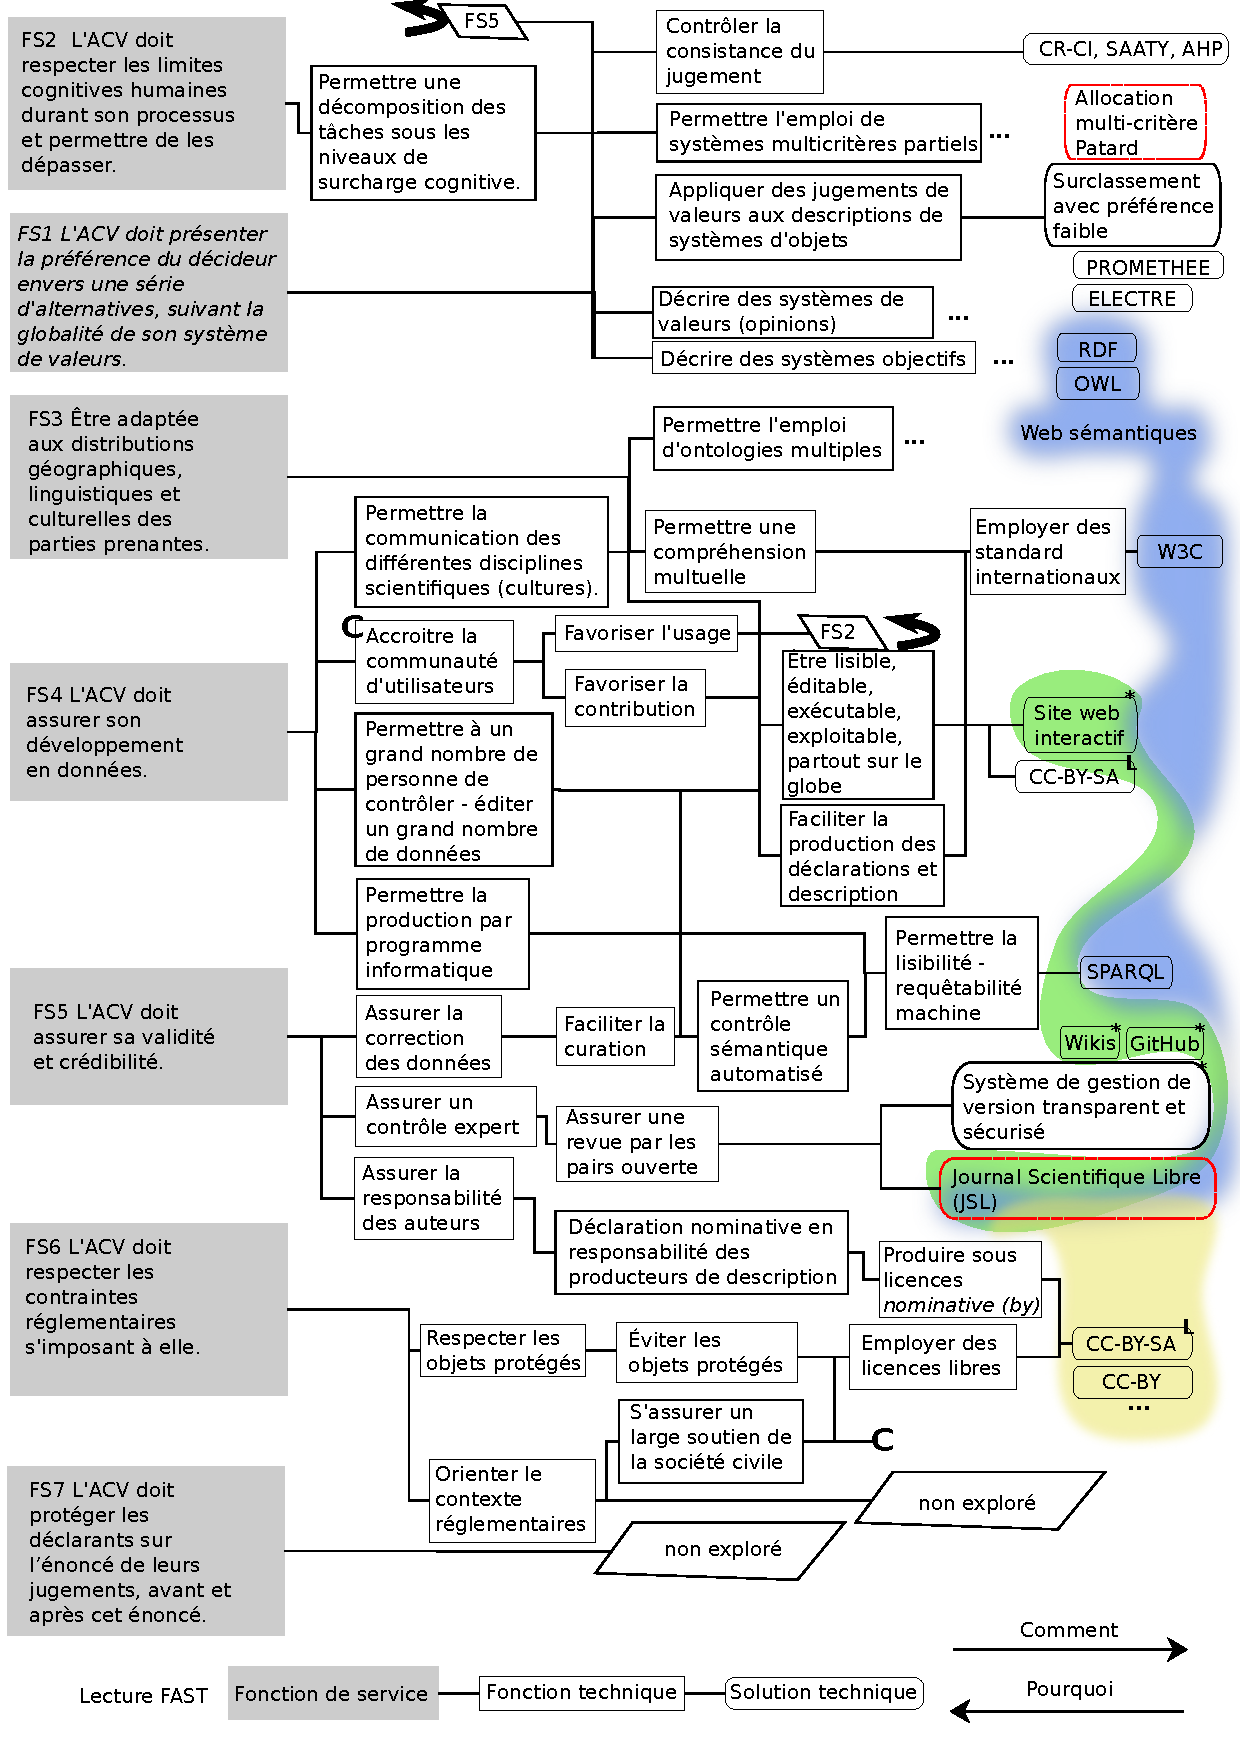
\includegraphics[width=\textwidth]{/home/rudy/Documents/rudy/01_These/11_production/01_COMMUNICATION/figures/FAST-fr_C.pdf}
  \caption{FAST}
  \label{fig:FAST_remix}
\end{figure}
\figbox{
Il apparaît lors de cette exploration des FAST combinés figure~\ref{fig:FAST_remix}, que des fonctions techniques sont communes à plusieurs fonctions de service.
Pour limiter le chargement de la figure de multiples traits additionnels et ne respectant pas les sens de lecture d'un diagramme FAST, nous procédons à des renvois par symbole.
\exbox{ex: ``S'assurer un large soutien de la société civile.'' \textsc{Comment}~?~: \textbf{C}, ``Accroître la communauté d'utilisateurs.''\ldots
``Contrôler la consistance du jugement'' \textsc{Pourquoi}~?~: ``FS5 L'ACV doit assurer sa validité et crédibilité.''\ldots}
En conséquence des solutions 'techniques' répondent à plusieurs fonctions.
Par exemple, le choix d'un système ouvert, transparent, avec gestion des versions et libre de droit, répond à de nombreuses contraintes sur l'adaptation aux parties prenantes, à la confiances pour celles-ci envers l'\gls{ACV} et dans le développement des données qui lui sont nécessaires (FS3 à FS6).

La question de la prise en compte des parties prenantes (en son sens le plus large FS1-3), tout en garantissant la protection des déclarants sur leur systèmes de valeurs (FS7) reprend des problématiques du vote électronique~\cite{enguehard_vote_2007,pellegrini_chaines_2014}.
Rappelons qu'il ne peut à la fois être garanti, que l'expression du jugement soit prise en compte \emph{et} que les expressions de jugements employées soient anonymes.
Il faut un procès de confiance.
Le recueil, pour les personnes souhaitant rester anonymes doit pouvoir être entré au système d'information par un tiers identifié et responsable de l'entrée de ces données nouvelles.
Sur un nombre vaste de dimensions, avec un nombre de combinaisons (valeurs de la matrice de jugement) d'importance relatives fortement supérieur au nombre de déclarant d'un groupe, il nous apparaît comme probable qu'un répondant puisse s'identifier au sein des systèmes de valeurs.
Ce point étant fortement éloigné de notre thématique initiale et de nos compétences, le soin en est laissé aux spécialistes de le poursuivre (Non-exploré).

Des évolutions législatives encours porte sur l'adaptation des administrations et de la gestion de données à l'ère des 'TIC' (République Numérique)~\cite{_republique_2015}.
Les délais d'embargo uniformisés entérinés par ce texte (bien que plus courts que ceux antérieurs~\cite{gouzi_loi_2016}), rendent délicat l'emploi d'une partie des données "fraîches" employables dans la part descriptives des systèmes observés.
Notamment sur les questions sociales où l'embargo est le plus long (12 mois), la nature des situations peut évoluer rapidement.
Par ailleurs, ces délais font obstacle à une procédure de vérification ouverte, repoussant encore le délai pour l'obtention d'une donnée validée ouvertement et par des pairs.
Une des orientations possibles pour certaines données de l'\gls{ACV} et le travail sous l'angle de l'exception de la recherche dans le domaine de la propriété (ex : exception pédagogique et de recherche~\cite{_droit_????}).
Elle se heurte toutefois à la multiplicité des législations et accords.
Or pour la recherche publique la voie reste libre à la libre publication comme développée au~\ref{sec:JSL}.
Une solution qu'il paraîtrait plus qu'inconsistant de la part de la recherche publique de ne pas employer.

Nous opérons la liaison des solutions de FS~1 ; FS~3-6 dans le journal scientifique libre, présentée au \ref{sec:JSL}.

}

À ce stade, si nous observons les fonctions requises, des solutions existantes apparaissent en littérature.


%For the respective requirement analysis,
%\begin{itemize}
% \item Application for decision,
% \item Dealing with multiple incommensurable attributes,
% \item Data intensive field, with data quality issues and continuous updates needed,
% \item Complex system representation that overwhelm individual human capacities.
%\end{itemize}
%
%
%PREFERENCE
%
%~\cite{these ADLA}
%~\cite{davis_making_2012}
%~\cite{sayan}
%~\cite{moullec_towards_2014}
%> clear depictions of MCDA as handling preferences. generally citing Roy and Bouyssou.
%The preference system being formalized around a limited set of criterionst}
%{Fonction de service}
%       \FT{FT1}
%       {
%         \FT{FT2}
%         {
%           \ST{Solution technique}
%         }
%       }
%       \FT{}
%       {
%         \FT{FT3}
%         {
%           \ST{ST2}
%         }
%       }
%       \FT{FT4}
%       {
%         \ST{ST3}
%       }
%{Fonction de service}
%       \FT{FT4}
%       {
%         \ST{ST3}
%       }
%       
%\end{fast}
%\fastReset
%
%This is what can be seen trough Rowley's work~\cite{rowley_aggregating_2012} as methods ``synthesising preference relational system'', in the classification of non-compensatory decision system, type 2 partial aggregation.
%
%Elements known before publication of ISO LCA standards: Roy, B., 1991. The outranking approach and the foundations of electre methods.
%Theory and Decision 31, 49e73.
%
%In literature we can find in isolation the different solutions.
%pass to table format
% \usepackage{multirow}

% \begin{landscape}
% \begin{table}[htbp]
%   \begin{center}
%   \caption{Characterization based on AF attributes Function, Criterion, Level, and current state in standard and practice.}
%   \begin{tabular}{|p{4cm}|p{4cm}|p{4cm}|p{3cm}|p{3cm}|}
%   \hline
%   Function&Criteria&Levels&Current state&Comments \\
%   \hline
%   \multirow{4}{*}{Enable the decision maker to select the option preferred} &Number of alternatives&Levels&Current state&Comments \\
%   &Criteria 2&Levels&Current state&Comments \\
%   &Criteria 2&Levels&Current state&Comments \\
%   &Criteria 2&Levels&Current state&Comments \\ \hline
%   \multirow{4}{*}{Encompass complexity of the system model} &Number of attributes&Levels&Current state&Comments \\
%   &Criteria 2&Levels&Current state&Comments \\
%   &Criteria 2&Levels&Current state&Comments \\
%   &Criteria 2&Levels&Current state&Comments \\ \hline
% 
%   \end{tabular}
%   \end{center}
%   \label{tab:Some solutions to already solved issue of LCA}
%   \end{table}
% \end{landscape}

%\begin{itemize}
% \item MCDA tools, ~\cite{rowley_aggregating_2012, herva_review_2013}
% \item Value expression, (here is a huge gap as the field reject value judgment).
% The occurrence found is about integrating judgment concluded \cite[Who would know better than this community about whether governments and industry sustainability measures are moving in the right direction and fast enough?]{freidberg_behind_2015},
% speaking of life cycle approach practitioners.
% But management's literature is more openly discussing those question.~\cite{berard_processus_2009}
% \footnote{To this matter of WHO should be stirring our society, choosing speed and direction, then I'd say EVERYBODY.
% Of course it is an opinion, but I'm not very pro a new fascism designed by a set of LCA specialists.}
% \item massively open and collaborative databases and software codes,
% \item semantic format for machine scalable application.
%\end{itemize}
%
%
%but sections dedicated to these part ?


\subsection{Observations des Pratiques et Normes}

La pratique de l'\gls{ACV} se réduit pour le moment à l'emploi majoritaire de codes fermés (\textit{cf.} \ref{subsec:L'interface de modélisation}), de données propriétaires diffusées en biens de club restreints (\textit{cf.} \ref{subsubsec:Bases de données}).
Les règles d'application se développent de façon sectorielle et compartimentée (normes, réglementation et déclaration, \gls{PCR}, \gls{EPD}) dans une certaine similitude au développement en recherche (\textit{cf.} \ref{subsec:Historique de la méthode, son développement, son contexte}).
Le tout alimente les secteurs entrepreneuriaux du conseil et de la normalisation (comme c'est le cas depuis la formalisation du domaine, \textit{cf.}~\ref{subsec:L'origine de l'ACV}).
L'ensemble invalide le cadre de développement des outils et des données de l'\gls{ACV}.


\paragraph{FS1} 
Présenter la préférence du décideur envers une série d'alternatives, suivant la globalité de son système de valeurs.

Actuellement, l'\textit{évaluation} réside dans la caractérisation, issue d'observation ET de jugements opérés de façon indépendants des interprétations finales.

À l'issue de la reconception, la sortie finale est un réseau hiérarchisé avec préférences flous d'alternatives en accord au système de valeur du décideur.

\paragraph{FS2} 
Respecter les limites cognitives humaines durant son processus et permettre de les dépasser.

Dans son état actuel, l'ACV repose sur des heuristiques d'application humaine à la sélection des indicateurs, à la détermination des unités fonctionnelles, à l'issue des résultats 'caractérisés'.
Les praticiens comme les 'clients' sont dans l'incapacité de réaliser le contrôle des jugements.
Ce qui n'est d'ailleurs même pas un soucie identifié par la communauté.

Après cette reconception, la capacité de contrôle de la consistance du jugement appliqué devient centrale.
Il y a réduction du nombre d'informations à post-traiter humainement sous le seuil de surcharge cognitive.

 
\paragraph{FS3} 
Être adaptée aux distributions géographiques, linguistiques et culturels des parties prenantes.

Localisation est pour le moment non-systématique.
La littérature est majoritairement anglophone.
Les jugements sont principalement occidentaux.
Quelques développements localisés existent sur les méthodes d'impacts (LUCAS, Canada ; LIME, Japon), non nécessairement traduits\footnote{\blockcquote{jrc_ilcd_2011}{ Information in non-Japanese language only partially available.}}.
Il n'y a pas d'information qui assiste l'application d'outils automatiques de traduction.
Pas de traitement des multiples orientations culturelles.
L'emploi de données spécifiques et à la charge justificatrice du praticien dans l'exception.

Après ce cycle de reconception la localisation des observations est systématique.
L'ouverture à la lecture et l'écriture permettent la traduction manuelle.
L'implémentation sémantique permet la traduction par script.
 
\paragraph{FS4} 
Assurer son développement en données.

C'est un problème récurant depuis la genèse jusqu'à l'état actuel.
Rien dans la méthodologie n'est posé pour sa résolution.
Des approches sémantiques sont en projets~\cite{weidema_bonsai_2014,vardeman_ontology_2015}, quelques données dans des bases sont libres en lectures.
 
Après reconception, les mécanismes de l’open-source associé à la production par scriptes font partie intégrante de la production en ACV.
La production d'évaluation est la résultante directe d'une interrogation de la base de connaissance depuis un système de valeur incluant des contraintes de qualité sur le matériel interrogé.


\paragraph{FS5} 
Assurer sa validité et crédibilité. 

La crédibilité de l'ACV est mise en défaut par une série de critiques non résolues et de multiple jugements de valeurs introduit dans la méthodologie.
La critique de la qualité des données et d'un traitement de l'incertitude n'est pas systématique aux études d'ACV.
Nous relevons une présence importante de donnée sans distribution\footnote{\blockcquote{mutel_why_2013}{ecoinvent 2.2 database Distribution Undefined	Technosphere~:~1629 ; Biosphere~:~37036}}.
Il y a de grande difficulté de traçabilité de la donnée.
 
De par notre reconception, le traitement des jugements de valeurs est identifié, isolé, explicite.
Les dépôts de données sont nominatifs, datés, localisés.
L'emploi des agrégations se fait par catégorie, sans "création" de données nouvelles (synthèse via la classification sémantique, via l'ontologie).
Le mécanisme de revue par les pairs par tag sémantique contribue à l'adéquation entre la qualité de l'information et les critère du décideur.
Il y a continuité de la responsabilité des auteurs.


\paragraph{FS6} 
Respecter les contraintes réglementaires s'imposant à elle.

Le copyright\textcopyright domine en présence. S'en suit le respect de la propriété de données majoritairement en 'biens de clubs' conduisant soit à l'inaccessibilité pour une vaste majorité des parties prenantes, soit par une violation des droits d'auteurs pour la consultation illégale.

Le reconception de l'ACV conduit à ce que les données soient systématiquement en open access.
Pas de copyright\textcopyright, donc pas de violation des droits de propriété lucrative.
Le contrôle sur les droits d'auteurs est possible par le contrôle de l'auteur du dépôt des descriptions des systèmes industriels ou environnementaux, ou des systèmes de valeurs anonymisés et collectifs recueilli par enquêtes (toutes les contributions sont nominatives). 
 
\paragraph{FS7} 
Protéger les déclarants sur l’énoncé de leurs jugements. 

L'absence des déclarations rend nul ce point dans l'état de l'art actuel.

Après reconception, l'anonymisation pour les requêtes via les systèmes de valeurs individuels est requise.
Il y a nécessité de protection pour le recueil des matrices collectives pour ne pas ciblé d'individu dans l'agrégat collectif.


%Confrontons donc de façon synthétique les caractéristiques décrites à l'issue de l'\gls{AF} et l'état actuel dans la table~\ref{tab:issue-actuel}.
%\begin{table}
%\begin{longtable}{|c|p{3cm}|p{4.5cm}|p{4.5cm}|}
%\hline
%Libellé & fonction & Issue \gls{AF} & État actuel\\
%\hline
%FS1 & Présenter la préférence du décideur envers une série d'alternatives, suivant la globalité de son système de valeurs.& Réseau hiérarchisé avec préférences flous d'alternatives en accord au système de valeur du décideur & Évaluation~: caractérisation issue d'observation ET de jugement opéré de façon indépendante des interprétations finales\\
%FS2 & Respecter les limites cognitives humaines durant son processus et permettre de les dépasser.& Capacité de contrôle de la consistance du jugement appliqué. Réduction du nombre d'informations à post-traiter humainement sous le seuil de surcharge cognitive. & Heuristiques d'application humaine à la sélection des indicateurs, à l'issue des résultats 'caractérisés'. Incapacité au contrôle des jugements\\
%FS3 & Être adaptée aux distributions géographiques, linguistiques et culturels des parties prenantes.& Localisation des observations systématique. Ouverture à la lecture et l'écriture permettant et donc la traduction manuelle. Implémentation sémantique permettant la traduction par script. J& Localisation non-systématique.  Littérature majoritairement anglophone, jugements occidentaux. Quelques développements localisés sur les méthodes d'impacts (LUCAS, Canada ; LIME, Japon), non nécessairement traduits\footnote{\blockcquote{jrc_ilcd_2011}{ Information in non-Japanese language only partially available.}}. Pas d'information assistant l'application d'outils automatiques de traduction. Pas de traitemendt des multiples orientations culturelles.\\
%FS4 & Assurer son développement en données.& Mécanismes de l’open-source associé à la production par scriptes & Problème récurant depuis la genèse jusqu'à l'état actuel. Approche sémantique en projets~\cite{weidema_bonsai_2014,vardeman_ontology_2015}. Quelques données dans des bases libres en lectures~\ref{subsect-bases_ouvertes, ex agribalise, carbone, impact}\\
%FS5 & Assurer sa validité et crédibilité. & Traitement des jugements de valeurs identifié, isolé, explicite. Dépôts de données nominatifs, datés, localisés, emploie des agrégations par catégorie sans "création" de données nouvelles (synthèse via la classification sémantique, l'ontologie). Mécanisme de revue par les pairs par tag sémantique. Continuité de la responsabilité des auteurs. & Critique non résolue de multiple jugements de valeurs introduit dans la méthodologie. Critique de la qualité des données et d'un traitement de l'incertitude non-systématique. Présence importante de donnée sans distribution\footnote{\blockcquote{mutel_why_2013}{ecoinvent 2.2 database Distribution Undefined	Technosphere~:~1629 ; Biosphere~:~37036}}. Difficulté de traçabilité de la donnée.\\
%FS6 & Respecter les contraintes réglementaires s'imposant à elle. & Données systématiquement en open access. Pas de \textcopyright, donc pas de violation des droit de propriété. Contrôle possible sur les droits d'auteurs par le contrôle de l'auteur du dépôt (nominatif). & \textcopyright, respect de la propriété de données majoritairement 'biens de clubs' conduisant soit à l'inaccessibilité pour une vaste majorité des parties prenantes, soit par une violation des droits d'auteurs pour la consultation illégale.\\
%FS7 & Protéger les déclarants sur l’énoncé de leurs jugements. & Anonymisation pour les requêtes via les systèmes de valeurs individuels. Nécessité de protection pour le recueil des matrices collectives. & Absence des déclaration prépondérante. Non concerné.\\
%\hline
%\caption{Confrontation état initial, reconception}
%\label{tab:final-actuel}
%\end{longtable}
%%\end{table}


\section{Approches complémentaires}
\subsection{Descriptif de l'application}
Nous (concepteur, pour ce que j'en ai été et côtoyé) rencontrons plus fréquemment les outils tel l'AMDEC et SAFE (\textit{cf.} le point~\ref{meth_conception}) sur des produits tangibles.
Mais pour l'exercice (que nous avons jugé utile de le relaté) observons ce que nous en tirons sur l'\gls{ACV}.

Pour identifier les défaillances qui peuvent survenir, nous commençons par développer une approche SAFE, puis AMDEC.
Nous ne prétendrons pas identifier systématiquement la fréquence ou la gravité mais nous pourrons commenter la capacité et probabilité de détection.
\subsection{Application}
\begin{itemize}
\item Première phase (but et périmètre).
\textit{SAFE.}
L'analyste définit avec l'utilisateur/décideur le système à étudier et le caractérise en vu de satisfaire un accroissement de performance.

Identifier le système de valeur permettant de définir la variation de performance.
Décideur et valeurs identifiables.

Mettre en relation analyste et utilisateur/décideur (ou réaliser leur identité).
Identité ou communication possible des deux corps.

Définir l'objet d'étude.
Objet circonscrit.

Caractériser l'objet d'étude.
Objet caractérisable.

\textit{AMDEC}
\begin{itemize}
\item Le décideur et son système de valeurs sont non ou mal identifiés/identifiable.
Le système de valeur est (i) incohérent (ii) sans légitimité axiologique pour les personnes subissant les conséquences.
\item Le décideur est clairement identifié mais (i) en opposition forte avec le système de valeur des populations subissant les conséquences (ii) craint de l'être (iii) craint une forte agitation de part les clivages sur les valeurs de la population concernée.
Le système de rationalisation est (i) rejeté pour ne pas expliciter le système de valeur employé (ii) masqué ou rendu non-transparent (retour au point précédent).

La capacité de détection réside dans la présence explicite du système de valeur avec des objets de contrôle de la consistance du jugement.
La détection binaire est donc aisé, la détection de défaut qualitatif l'est moins.
Quant à la probabilité, l'ACV a une génération derrière elle sans que cette part critique du système de décision lui soit réclamée.
La capacité aisé n’entraîne donc pas la réalisation ni la mise en place effective du contrôle.

\item La perception fonctionnelle du système de premier plan observé est (i) incomplète (incertitude épistémologique ou absence d'étude antérieur).
Les confrontations d'alternatives ne se démarquent pas sur le plan fonctionnelle, les conclusions en sont maintenues à l'ordre de l’indifférence ou de l'incomparabilité.
Une répétition de ce cas entraîne un renforcement opérant négatif et donc le rejet de la méthode.

Il faut une grande connaissance des systèmes observés pour réaliser que la description de ceux-ci sont incomplets et cela dans une mesure suffisamment critique pour invalider une itération de l'étude d'ACV.
L'absence de détection peut conduire à une prescription erroné quant à l'alternative effectivement préférée.
Même détecter les limitations organisationnelle et économique (temps, ressources) peuvent être fatales (absence de décision suivant la méthodologie).

\end{itemize}
\item Inventaire.
\textit{SAFE.}
Compléter la description du système étudié (premier plan et arrière plan affecter), respectivement au domaine informationnel réclamé par le système de valeur du décideur.

Décrire les procédés unitaires.
Procédés descriptibles.

Recevoir, stocker, traiter, transmettre de l'information (non-développé, séquence classique des systèmes d'information).

\textit{AMDEC}
\begin{itemize}
\item Il s'agit ici des défaillances de traitement de l'information et du signal.
Nous ne les développons pas toutes (bruits, incertitudes de mesures).
\item Problème ou absence de traçabilité (méta-données).
S'il s'agit d'antériorité sans réplication possible, la gravité est forte puisqu'il s'agit d'éléments qui resteront inconnu.
Un caractère incomplet sur des informations fortement appréciée du décideur (importante dans son système de valeur) peuvent rendre caduque l'exercice.
\item Incapacité à intégrer des pièces (chunks) d'information nouvelles.
Cela peut provenir d'un problème technique (format de donnée) ou réglementaire (fermeture légal de l'exploitation des données).
Est associé à ce point l'incohérence ontologique.
\exbox{Une désignation de flux sans correspondance avec les systèmes voisins, qu'ils soient techniques ou environnementaux.
Ex : Un compartiment 'Bassin méditerranéen' pour une méthode ne disposant que des compartiments génériques sol, air, eau ; COV, VS décomposition par espèce de composé organique ; Particule totale VS PM10, PM2.5 VS surface spécifique ; un système industriel consommant (ou appelant en nomenclature) un composant exprimé en DIN pour un système lisant des désignations NF etc.}
\item Taille du système à inventorier dépassant les capacités des acteurs.
Au regard de la globalité (planète) du système en question, nous pouvons dire sur la fréquence qu'elle est systématique en l'absence de mutualisations vastes.
La détection n'est pas systématiquement évidente.
Il pourrait y avoir des plateaux de convergence locaux d'inventaire.
Sur la question de la fréquence de rafraîchissement des outils correctifs de l'incertitude existent telle la "pedigree matrix"~\cite{weidema_data_1996}. La critique des systèmes d'évaluation et la correction d'écart-type apportée doit évidement être réalisée, développée, mise-à-jour.
\end{itemize}
\item Interprétation.
Nous considérons les problématiques de documentation des méthodes d'impacts comme celle de la documentation des procédés environnementaux, c.a.d. comme relevant de l'inventaire.
L'interprétation vise donc le jugement.

\textit{SAFE}
Appliquer le système de valeur du décideur aux descriptions du système et des alternatives pour produire la décision.
(Sous décomposition suivant \gls{ADMC}.)

ADMC appropriable par le(s) décideur(s).

\textit{AMDEC}
\begin{itemize}
\item Inadéquation de la méthode de traitement et du système de valeur.
La détection nécessite que l'usager et/ou le décisionnaire ait une bonne maîtrise (i) du système de valeur, (ii) des \gls{ADMC} correspondantes.
Les inadéquations observées sont fréquentes si ce n'est systématique.
Même s'il y a correspondance, le rejet potentiel de la complexité intrinsèque des méthodes peut entraîner leur rejet par le décideur.
Leur emploi (et donc celui de l'\gls{ACV}) est donc potentiellement conditionné par l'apprentissage et la formation (ou l’acculturation) du décideur aux méthodes d'\gls{ADMC}
\item Temps de calcul qui excède la temporalité de la décision.
De part l'incertitude des délais de réponse, il n'est pas à exclure qu'il faille, pour des cas opérationnelle, également considérer l'emploi d'heuristique et de processus hiérarchique autoritaire.
Indépendamment de la réduction du temps de calcul à des niveaux acceptés (acceptables), il peut y a voir rejet des ADMC par le décideur par un sentiment de confiscation du pouvoir décisionnel sur les questions de moyen et long termes (délai long accessible pour le calcul).
La maîtrise de la temporalité des cadres décisionnelles est donc importante pour les parties-prenantes.
\end{itemize}
\end{itemize}

Concernant l'\emph{Examen des mouvements et des efforts} (\textit{cf.} sec.\ref{subsubsec:RÉSEAU}), nous relevons que l'effort qui semble être le plus important réside dans l'abandon d'une heuristique rapide au système de valeur implicite permettant au décideur de se maintenir dans un confort cognitif et psychologique.
\blockcquote[traduction]{murray_transdisciplinary_2015}{Si le temps et l'effort cognitif sont limités, alors les modèles à double processus de persuasion suggèrent que les heuristiques seront utilisés dans la prise de décision (Vaughan et Hogg 2011).}
%If time and cognitive effort is limited, then dual-process models of persuasion suggest that heuristics will be used in decision making (Vaughan and Hogg 2011).
%}
L'impression de maîtrise du décideur dominant, son sentiment d'avoir 'maximiser' sa performance même concernant des valeurs controversées parce qu'il n'a pas à expliciter l'ensemble des critères et leur importance relative est un obstacle en \gls{ACV} comme pour l'ensemble des \gls{ADMC}.


L'énoncer, "faciliter la renonciation à la solution \emph{intuitivement meilleure}" serait sans doute une fonction de plus à ajouter à notre artefact.
Mais nous laisserons cela aux psychologues pour le moment.

\subsection{Synthèse de l'apport des approches complémentaires}
Nous observons des caractères similaires à l'\gls{AF}, tel le caractère inter-opérable des ontologies à employer.
Ce qui ressort de façon plus saillante qu'avec l'outil de conception précédent, c'est l'adéquation et l'acceptabilité du système de décision et sa complexité.
La capacité à la reconnaissance explicite d'un système de valeur et la renonciation à une heuristique intuitive pour la prise de décision sont des points sensibles.
\section{Re-conception de l'ACV, conclusion et perspective}
\label{sec:Re-conception de l'ACV, conclusion et perspective}
%\begin{center}\colorbox{blue}{-- Traduction --}\end{center}

%En fait c'est plus part sérenpidité\footnote{} et adbuction\footnote{} que je suis venu au conclusion précédentes.
%En effet à la lecture au début de mon doctorat de l'article de John Reap\cite{reap_survey_2008}, c'est la notation en exposant d'un petit "a" et de la note indicative qui m'a ouvert les yeux.
%\blockcquote{reap_survey_2008}{problematic decision}
Nous aurons durant ce parcours pu observer les zones de recouvrement entre \gls{ACV}, \gls{ADMC}, conceptual design methods (CDM).
En effet, toutes les applications relevant de l'\emph{évaluation} comportent des racines communes.
La caractéristique centrale de l'\gls{ACV} concerne le contrôle du report dimensionnelle et tend vers l'holisme (\textit{cf.} section \ref{sec:La pensée en cycle de vie}).
Remplacer '\gls{ACV}' par 'évaluation holistique' produirait certainement un résultat d'analyse fonctionnelle similaire.

Certains des principes énoncés sont donc non seulement valide pour la pensée en cycle de vie mais aussi plus généralement pour la pratique de l'évaluation pour une rationalité accrue.

Cette analyse fait ressortir les trois éléments anticipés dans nos travaux initiaux~\cite{patard_life_2015} et qui constituent la colonne vertébrale de cette production~:
\begin{itemize}
\item L'intégration du jugement du décideur pour respecter le caractère intrinsèque de l'é\emph{valuation}.
\item L'emploi des techniques d'aide à la décision multicritère pour rester sous la surcharge cognitive \textbf{et} étendre notre capacité à la rationalité.
\item L'ouverture des données, méthodes et outils pour faire face au caractère intensif en données de la discipline.
\end{itemize}

Deux éléments complémentaires sont issues de la démarche d'\gls{AF}.
\begin{itemize}
\item La question de la protection du déclarant à laquelle nous ne prêtions pas d'attention antérieurement est également soulignée.
\item Initialement pensée sur la compatibilité des langages informatiques et techniques, la question des ontologies a élargie la question de l'interaction \emph{disciplinaire} à l'interaction et à la diversité \emph{culturelle}.
\end{itemize}

Les approches complémentaires tel l'AMDEC nous aurons apporté des éléments critiques sur l'\emph{acceptabilité} d'un système d'aide à la décision complexe avec système de valeur explicite.
Ces approches mettent à jours une dimension psychologique de la renonciation aux heuristiques autoritaires non assistées.

La confrontation de l'analyse fonctionnelle aux guides et normes actuels souligne l'importance du manque de l'intégration du jugement de valeur du décideur dans cette méthodologie d'évaluation.
Les approches complémentaires nous éclairent également sur des raisons possible à cette absence.
Nous réitérons ici la proposition (\textit{cf.} figure~\ref{fig:ILCD-V2} en annexe~\ref{sec:Un nouveau standard}) d’entamer la révision de la série ISO~14040 et de l'ILCD par l'introduction d'une \emph{étape d'intégration explicite du jugement de valeurs} au sein d'une norme ouverte~\cite{patard_life_2015}.

La méthode de conception principale que nous avons sélectionnée n'est pas exempte de critique~\cite{darses_francoise_assister_2001}.
Notre communauté, plus particulièrement ses membres dans le domaine de la conception, est donc invitée à produire des analyses alternatives. %(via PSARE par exemple)
Confirmer ou infirmer le diagnostic fonctionnelle de l'objet \gls{ACV} est important afin de produire à l'avenir un outil efficace mais aussi de plus grande robustesse, acceptabilité et légitimité.
%\footnote{Our community, more particularly those in design field, is of course invited to produce alternative analysis to produce confirmation or infirm the following elements.}

%To fully describe how I came to this perspective consider the following statements.
%What John Reap classifies as pivotal decisions are modeling choices of the LCA practitioner.
%So consider each ``problematic decision'' practitioners have to make and discuss them.
% 
% ? considering using text analysis to apply NLTK and search for stem of each question perimeter.
% vocabulary of the section:
% \begin{itemize}
%  \item Functional unit
%  \item function
%  \item reference flow
%  \item multifunctional / multi-functional / coproduct
% \end{itemize}

% \paragraph{

